% Created by tikzDevice version 0.6.1 on 2016-04-19 16:54:45
% !TEX encoding = UTF-8 Unicode
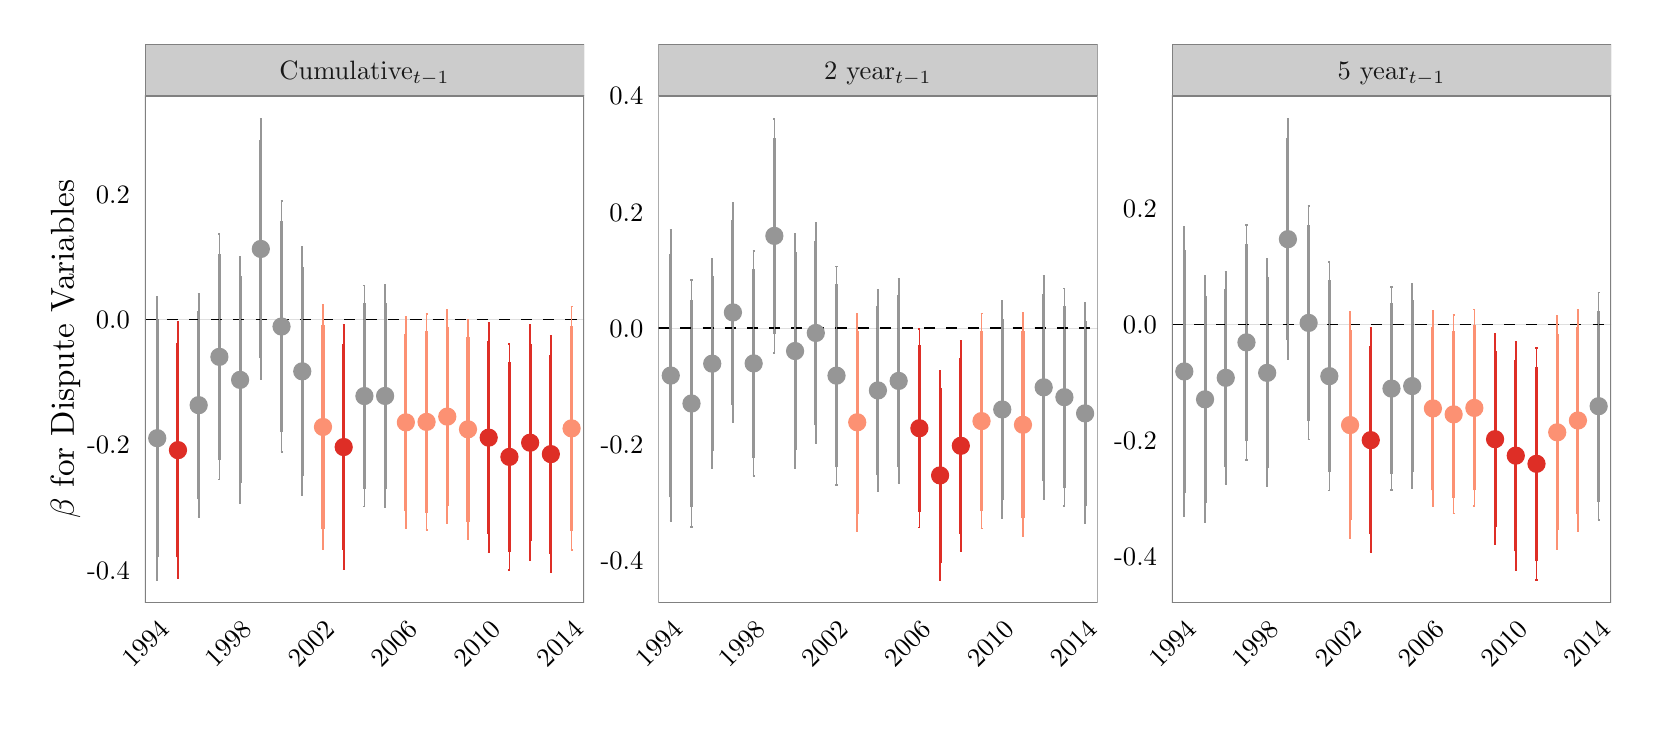
\begin{tikzpicture}[x=1pt,y=1pt]
\definecolor[named]{drawColor}{rgb}{0.00,0.00,0.00}
\definecolor[named]{fillColor}{rgb}{1.00,1.00,1.00}
\fill[color=fillColor,] (0,0) rectangle (578.16,252.94);
\begin{scope}
\path[clip] (  0.00,  0.00) rectangle (578.16,252.94);
\definecolor[named]{fillColor}{rgb}{0.00,0.00,0.00}
\end{scope}
\begin{scope}
\path[clip] (  0.00,  0.00) rectangle (578.16,252.94);
\definecolor[named]{fillColor}{rgb}{0.00,0.00,0.00}
\end{scope}
\begin{scope}
\path[clip] (  0.00,  0.00) rectangle (578.16,252.94);
\definecolor[named]{fillColor}{rgb}{0.00,0.00,0.00}
\end{scope}
\begin{scope}
\path[clip] (  0.00,  0.00) rectangle (578.16,252.94);
\definecolor[named]{fillColor}{rgb}{0.00,0.00,0.00}
\end{scope}
\begin{scope}
\path[clip] (  0.00,  0.00) rectangle (578.16,252.94);
\definecolor[named]{fillColor}{rgb}{0.00,0.00,0.00}
\end{scope}
\begin{scope}
\path[clip] (  0.00,  0.00) rectangle (578.16,252.94);
\definecolor[named]{fillColor}{rgb}{0.00,0.00,0.00}
\end{scope}
\begin{scope}
\path[clip] (  0.00,  0.00) rectangle (578.16,252.94);
\definecolor[named]{fillColor}{rgb}{0.00,0.00,0.00}
\end{scope}
\begin{scope}
\path[clip] (  0.00,  0.00) rectangle (578.16,252.94);
\definecolor[named]{fillColor}{rgb}{0.00,0.00,0.00}
\end{scope}
\begin{scope}
\path[clip] (  0.00,  0.00) rectangle (578.16,252.94);
\definecolor[named]{fillColor}{rgb}{0.00,0.00,0.00}
\end{scope}
\begin{scope}
\path[clip] (  0.00,  0.00) rectangle (578.16,252.94);
\definecolor[named]{fillColor}{rgb}{0.00,0.00,0.00}
\end{scope}
\begin{scope}
\path[clip] (  0.00,  0.00) rectangle (578.16,252.94);
\definecolor[named]{fillColor}{rgb}{0.00,0.00,0.00}
\end{scope}
\begin{scope}
\path[clip] (  0.00,  0.00) rectangle (578.16,252.94);
\definecolor[named]{fillColor}{rgb}{0.00,0.00,0.00}
\end{scope}
\begin{scope}
\path[clip] (  0.00,  0.00) rectangle (578.16,252.94);
\definecolor[named]{fillColor}{rgb}{0.00,0.00,0.00}
\end{scope}
\begin{scope}
\path[clip] (  0.00,  0.00) rectangle (578.16,252.94);
\definecolor[named]{fillColor}{rgb}{0.00,0.00,0.00}
\end{scope}
\begin{scope}
\path[clip] (  0.00,  0.00) rectangle (578.16,252.94);
\definecolor[named]{fillColor}{rgb}{0.00,0.00,0.00}
\end{scope}
\begin{scope}
\path[clip] (  0.00,  0.00) rectangle (578.16,252.94);
\definecolor[named]{fillColor}{rgb}{0.00,0.00,0.00}
\end{scope}
\begin{scope}
\path[clip] (  0.00,  0.00) rectangle (578.16,252.94);
\definecolor[named]{fillColor}{rgb}{0.00,0.00,0.00}
\end{scope}
\begin{scope}
\path[clip] (  0.00,  0.00) rectangle (578.16,252.94);
\definecolor[named]{fillColor}{rgb}{0.00,0.00,0.00}
\end{scope}
\begin{scope}
\path[clip] (  0.00,  0.00) rectangle (578.16,252.94);
\definecolor[named]{fillColor}{rgb}{0.00,0.00,0.00}
\definecolor[named]{drawColor}{rgb}{1.00,1.00,1.00}
\definecolor[named]{fillColor}{rgb}{1.00,1.00,1.00}

\draw[color=drawColor,line width= 0.6pt,line cap=round,line join=round,fill=fillColor,] ( -0.00,  0.00) rectangle (578.16,252.94);
\end{scope}
\begin{scope}
\path[clip] (  0.00,  0.00) rectangle (578.16,252.94);
\definecolor[named]{fillColor}{rgb}{0.00,0.00,0.00}
\end{scope}
\begin{scope}
\path[clip] ( 42.33, 45.11) rectangle (201.03,228.33);
\definecolor[named]{fillColor}{rgb}{0.00,0.00,0.00}
\definecolor[named]{fillColor}{rgb}{1.00,1.00,1.00}

\draw[fill=fillColor,draw opacity=0.00,] ( 42.33, 45.11) rectangle (201.03,228.33);
\definecolor[named]{drawColor}{rgb}{0.59,0.59,0.59}
\definecolor[named]{fillColor}{rgb}{0.59,0.59,0.59}

\draw[color=drawColor,line width= 0.3pt,line join=round,fill=fillColor,fill opacity=0.30,draw opacity=0.30,] ( 46.82, 53.44) -- ( 46.82,155.76);
\definecolor[named]{drawColor}{rgb}{0.87,0.18,0.15}
\definecolor[named]{fillColor}{rgb}{0.87,0.18,0.15}

\draw[color=drawColor,line width= 0.3pt,line join=round,fill=fillColor,fill opacity=0.30,draw opacity=0.30,] ( 54.31, 54.07) -- ( 54.31,146.49);
\definecolor[named]{drawColor}{rgb}{0.59,0.59,0.59}
\definecolor[named]{fillColor}{rgb}{0.59,0.59,0.59}

\draw[color=drawColor,line width= 0.3pt,line join=round,fill=fillColor,fill opacity=0.30,draw opacity=0.30,] ( 61.79, 76.13) -- ( 61.79,156.92);

\draw[color=drawColor,line width= 0.3pt,line join=round,fill=fillColor,fill opacity=0.30,draw opacity=0.30,] ( 69.28, 89.61) -- ( 69.28,178.36);

\draw[color=drawColor,line width= 0.3pt,line join=round,fill=fillColor,fill opacity=0.30,draw opacity=0.30,] ( 76.76, 81.15) -- ( 76.76,170.20);

\draw[color=drawColor,line width= 0.3pt,line join=round,fill=fillColor,fill opacity=0.30,draw opacity=0.30,] ( 84.25,125.96) -- ( 84.25,220.01);

\draw[color=drawColor,line width= 0.3pt,line join=round,fill=fillColor,fill opacity=0.30,draw opacity=0.30,] ( 91.73, 99.51) -- ( 91.73,190.40);

\draw[color=drawColor,line width= 0.3pt,line join=round,fill=fillColor,fill opacity=0.30,draw opacity=0.30,] ( 99.22, 83.89) -- ( 99.22,173.61);
\definecolor[named]{drawColor}{rgb}{0.99,0.57,0.45}
\definecolor[named]{fillColor}{rgb}{0.99,0.57,0.45}

\draw[color=drawColor,line width= 0.3pt,line join=round,fill=fillColor,fill opacity=0.30,draw opacity=0.30,] (106.71, 64.53) -- (106.71,152.76);
\definecolor[named]{drawColor}{rgb}{0.87,0.18,0.15}
\definecolor[named]{fillColor}{rgb}{0.87,0.18,0.15}

\draw[color=drawColor,line width= 0.3pt,line join=round,fill=fillColor,fill opacity=0.30,draw opacity=0.30,] (114.19, 57.21) -- (114.19,145.59);
\definecolor[named]{drawColor}{rgb}{0.59,0.59,0.59}
\definecolor[named]{fillColor}{rgb}{0.59,0.59,0.59}

\draw[color=drawColor,line width= 0.3pt,line join=round,fill=fillColor,fill opacity=0.30,draw opacity=0.30,] (121.68, 79.91) -- (121.68,159.75);

\draw[color=drawColor,line width= 0.3pt,line join=round,fill=fillColor,fill opacity=0.30,draw opacity=0.30,] (129.16, 79.81) -- (129.16,159.92);
\definecolor[named]{drawColor}{rgb}{0.99,0.57,0.45}
\definecolor[named]{fillColor}{rgb}{0.99,0.57,0.45}

\draw[color=drawColor,line width= 0.3pt,line join=round,fill=fillColor,fill opacity=0.30,draw opacity=0.30,] (136.65, 72.07) -- (136.65,148.54);

\draw[color=drawColor,line width= 0.3pt,line join=round,fill=fillColor,fill opacity=0.30,draw opacity=0.30,] (144.14, 71.45) -- (144.14,149.50);

\draw[color=drawColor,line width= 0.3pt,line join=round,fill=fillColor,fill opacity=0.30,draw opacity=0.30,] (151.62, 73.73) -- (151.62,151.06);

\draw[color=drawColor,line width= 0.3pt,line join=round,fill=fillColor,fill opacity=0.30,draw opacity=0.30,] (159.11, 68.11) -- (159.11,147.49);
\definecolor[named]{drawColor}{rgb}{0.87,0.18,0.15}
\definecolor[named]{fillColor}{rgb}{0.87,0.18,0.15}

\draw[color=drawColor,line width= 0.3pt,line join=round,fill=fillColor,fill opacity=0.30,draw opacity=0.30,] (166.59, 63.33) -- (166.59,146.27);

\draw[color=drawColor,line width= 0.3pt,line join=round,fill=fillColor,fill opacity=0.30,draw opacity=0.30,] (174.08, 56.95) -- (174.08,138.73);

\draw[color=drawColor,line width= 0.3pt,line join=round,fill=fillColor,fill opacity=0.30,draw opacity=0.30,] (181.57, 60.55) -- (181.57,145.39);

\draw[color=drawColor,line width= 0.3pt,line join=round,fill=fillColor,fill opacity=0.30,draw opacity=0.30,] (189.05, 56.01) -- (189.05,141.66);
\definecolor[named]{drawColor}{rgb}{0.99,0.57,0.45}
\definecolor[named]{fillColor}{rgb}{0.99,0.57,0.45}

\draw[color=drawColor,line width= 0.3pt,line join=round,fill=fillColor,fill opacity=0.30,draw opacity=0.30,] (196.54, 64.08) -- (196.54,152.20);
\definecolor[named]{drawColor}{rgb}{0.59,0.59,0.59}
\definecolor[named]{fillColor}{rgb}{0.59,0.59,0.59}

\draw[color=drawColor,line width= 1.1pt,line join=round,fill=fillColor,] ( 46.82, 61.67) -- ( 46.82,147.54);
\definecolor[named]{drawColor}{rgb}{0.87,0.18,0.15}
\definecolor[named]{fillColor}{rgb}{0.87,0.18,0.15}

\draw[color=drawColor,line width= 1.1pt,line join=round,fill=fillColor,] ( 54.31, 61.49) -- ( 54.31,139.06);
\definecolor[named]{drawColor}{rgb}{0.59,0.59,0.59}
\definecolor[named]{fillColor}{rgb}{0.59,0.59,0.59}

\draw[color=drawColor,line width= 1.1pt,line join=round,fill=fillColor,] ( 61.79, 82.62) -- ( 61.79,150.43);

\draw[color=drawColor,line width= 1.1pt,line join=round,fill=fillColor,] ( 69.28, 96.75) -- ( 69.28,171.23);

\draw[color=drawColor,line width= 1.1pt,line join=round,fill=fillColor,] ( 76.76, 88.31) -- ( 76.76,163.04);

\draw[color=drawColor,line width= 1.1pt,line join=round,fill=fillColor,] ( 84.25,133.52) -- ( 84.25,212.45);

\draw[color=drawColor,line width= 1.1pt,line join=round,fill=fillColor,] ( 91.73,106.81) -- ( 91.73,183.09);

\draw[color=drawColor,line width= 1.1pt,line join=round,fill=fillColor,] ( 99.22, 91.11) -- ( 99.22,166.40);
\definecolor[named]{drawColor}{rgb}{0.99,0.57,0.45}
\definecolor[named]{fillColor}{rgb}{0.99,0.57,0.45}

\draw[color=drawColor,line width= 1.1pt,line join=round,fill=fillColor,] (106.71, 71.62) -- (106.71,145.67);
\definecolor[named]{drawColor}{rgb}{0.87,0.18,0.15}
\definecolor[named]{fillColor}{rgb}{0.87,0.18,0.15}

\draw[color=drawColor,line width= 1.1pt,line join=round,fill=fillColor,] (114.19, 64.32) -- (114.19,138.49);
\definecolor[named]{drawColor}{rgb}{0.59,0.59,0.59}
\definecolor[named]{fillColor}{rgb}{0.59,0.59,0.59}

\draw[color=drawColor,line width= 1.1pt,line join=round,fill=fillColor,] (121.68, 86.33) -- (121.68,153.33);

\draw[color=drawColor,line width= 1.1pt,line join=round,fill=fillColor,] (129.16, 86.25) -- (129.16,153.48);
\definecolor[named]{drawColor}{rgb}{0.99,0.57,0.45}
\definecolor[named]{fillColor}{rgb}{0.99,0.57,0.45}

\draw[color=drawColor,line width= 1.1pt,line join=round,fill=fillColor,] (136.65, 78.22) -- (136.65,142.40);

\draw[color=drawColor,line width= 1.1pt,line join=round,fill=fillColor,] (144.14, 77.72) -- (144.14,143.23);

\draw[color=drawColor,line width= 1.1pt,line join=round,fill=fillColor,] (151.62, 79.94) -- (151.62,144.85);

\draw[color=drawColor,line width= 1.1pt,line join=round,fill=fillColor,] (159.11, 74.49) -- (159.11,141.11);
\definecolor[named]{drawColor}{rgb}{0.87,0.18,0.15}
\definecolor[named]{fillColor}{rgb}{0.87,0.18,0.15}

\draw[color=drawColor,line width= 1.1pt,line join=round,fill=fillColor,] (166.59, 70.00) -- (166.59,139.60);

\draw[color=drawColor,line width= 1.1pt,line join=round,fill=fillColor,] (174.08, 63.52) -- (174.08,132.16);

\draw[color=drawColor,line width= 1.1pt,line join=round,fill=fillColor,] (181.57, 67.37) -- (181.57,138.57);

\draw[color=drawColor,line width= 1.1pt,line join=round,fill=fillColor,] (189.05, 62.90) -- (189.05,134.78);
\definecolor[named]{drawColor}{rgb}{0.99,0.57,0.45}
\definecolor[named]{fillColor}{rgb}{0.99,0.57,0.45}

\draw[color=drawColor,line width= 1.1pt,line join=round,fill=fillColor,] (196.54, 71.16) -- (196.54,145.11);
\definecolor[named]{drawColor}{rgb}{0.00,0.00,0.00}
\definecolor[named]{fillColor}{rgb}{0.00,0.00,0.00}

\draw[color=drawColor,line width= 0.6pt,dash pattern=on 4pt off 4pt ,line join=round,fill=fillColor,] ( 42.33,147.44) -- (201.03,147.44);
\definecolor[named]{drawColor}{rgb}{0.59,0.59,0.59}
\definecolor[named]{fillColor}{rgb}{0.59,0.59,0.59}

\draw[color=drawColor,line width= 0.4pt,line cap=round,line join=round,fill=fillColor,] ( 46.82,104.60) circle (  3.09);
\definecolor[named]{drawColor}{rgb}{0.87,0.18,0.15}
\definecolor[named]{fillColor}{rgb}{0.87,0.18,0.15}

\draw[color=drawColor,line width= 0.4pt,line cap=round,line join=round,fill=fillColor,] ( 54.31,100.28) circle (  3.09);
\definecolor[named]{drawColor}{rgb}{0.59,0.59,0.59}
\definecolor[named]{fillColor}{rgb}{0.59,0.59,0.59}

\draw[color=drawColor,line width= 0.4pt,line cap=round,line join=round,fill=fillColor,] ( 61.79,116.53) circle (  3.09);

\draw[color=drawColor,line width= 0.4pt,line cap=round,line join=round,fill=fillColor,] ( 69.28,133.99) circle (  3.09);

\draw[color=drawColor,line width= 0.4pt,line cap=round,line join=round,fill=fillColor,] ( 76.76,125.67) circle (  3.09);

\draw[color=drawColor,line width= 0.4pt,line cap=round,line join=round,fill=fillColor,] ( 84.25,172.98) circle (  3.09);

\draw[color=drawColor,line width= 0.4pt,line cap=round,line join=round,fill=fillColor,] ( 91.73,144.95) circle (  3.09);

\draw[color=drawColor,line width= 0.4pt,line cap=round,line join=round,fill=fillColor,] ( 99.22,128.75) circle (  3.09);
\definecolor[named]{drawColor}{rgb}{0.99,0.57,0.45}
\definecolor[named]{fillColor}{rgb}{0.99,0.57,0.45}

\draw[color=drawColor,line width= 0.4pt,line cap=round,line join=round,fill=fillColor,] (106.71,108.65) circle (  3.09);
\definecolor[named]{drawColor}{rgb}{0.87,0.18,0.15}
\definecolor[named]{fillColor}{rgb}{0.87,0.18,0.15}

\draw[color=drawColor,line width= 0.4pt,line cap=round,line join=round,fill=fillColor,] (114.19,101.40) circle (  3.09);
\definecolor[named]{drawColor}{rgb}{0.59,0.59,0.59}
\definecolor[named]{fillColor}{rgb}{0.59,0.59,0.59}

\draw[color=drawColor,line width= 0.4pt,line cap=round,line join=round,fill=fillColor,] (121.68,119.83) circle (  3.09);

\draw[color=drawColor,line width= 0.4pt,line cap=round,line join=round,fill=fillColor,] (129.16,119.86) circle (  3.09);
\definecolor[named]{drawColor}{rgb}{0.99,0.57,0.45}
\definecolor[named]{fillColor}{rgb}{0.99,0.57,0.45}

\draw[color=drawColor,line width= 0.4pt,line cap=round,line join=round,fill=fillColor,] (136.65,110.31) circle (  3.09);

\draw[color=drawColor,line width= 0.4pt,line cap=round,line join=round,fill=fillColor,] (144.14,110.48) circle (  3.09);

\draw[color=drawColor,line width= 0.4pt,line cap=round,line join=round,fill=fillColor,] (151.62,112.40) circle (  3.09);

\draw[color=drawColor,line width= 0.4pt,line cap=round,line join=round,fill=fillColor,] (159.11,107.80) circle (  3.09);
\definecolor[named]{drawColor}{rgb}{0.87,0.18,0.15}
\definecolor[named]{fillColor}{rgb}{0.87,0.18,0.15}

\draw[color=drawColor,line width= 0.4pt,line cap=round,line join=round,fill=fillColor,] (166.59,104.80) circle (  3.09);

\draw[color=drawColor,line width= 0.4pt,line cap=round,line join=round,fill=fillColor,] (174.08, 97.84) circle (  3.09);

\draw[color=drawColor,line width= 0.4pt,line cap=round,line join=round,fill=fillColor,] (181.57,102.97) circle (  3.09);

\draw[color=drawColor,line width= 0.4pt,line cap=round,line join=round,fill=fillColor,] (189.05, 98.84) circle (  3.09);
\definecolor[named]{drawColor}{rgb}{0.99,0.57,0.45}
\definecolor[named]{fillColor}{rgb}{0.99,0.57,0.45}

\draw[color=drawColor,line width= 0.4pt,line cap=round,line join=round,fill=fillColor,] (196.54,108.14) circle (  3.09);
\definecolor[named]{drawColor}{rgb}{0.59,0.59,0.59}
\definecolor[named]{fillColor}{rgb}{0.59,0.59,0.59}

\draw[color=drawColor,line width= 0.6pt,line join=round,] ( 46.44,155.76) --
	( 47.19,155.76);

\draw[color=drawColor,line width= 0.6pt,line join=round,] ( 46.82,155.76) --
	( 46.82, 53.44);

\draw[color=drawColor,line width= 0.6pt,line join=round,] ( 46.44, 53.44) --
	( 47.19, 53.44);
\definecolor[named]{drawColor}{rgb}{0.87,0.18,0.15}
\definecolor[named]{fillColor}{rgb}{0.87,0.18,0.15}

\draw[color=drawColor,line width= 0.6pt,line join=round,] ( 53.93,146.49) --
	( 54.68,146.49);

\draw[color=drawColor,line width= 0.6pt,line join=round,] ( 54.31,146.49) --
	( 54.31, 54.07);

\draw[color=drawColor,line width= 0.6pt,line join=round,] ( 53.93, 54.07) --
	( 54.68, 54.07);
\definecolor[named]{drawColor}{rgb}{0.59,0.59,0.59}
\definecolor[named]{fillColor}{rgb}{0.59,0.59,0.59}

\draw[color=drawColor,line width= 0.6pt,line join=round,] ( 61.42,156.92) --
	( 62.17,156.92);

\draw[color=drawColor,line width= 0.6pt,line join=round,] ( 61.79,156.92) --
	( 61.79, 76.13);

\draw[color=drawColor,line width= 0.6pt,line join=round,] ( 61.42, 76.13) --
	( 62.17, 76.13);

\draw[color=drawColor,line width= 0.6pt,line join=round,] ( 68.90,178.36) --
	( 69.65,178.36);

\draw[color=drawColor,line width= 0.6pt,line join=round,] ( 69.28,178.36) --
	( 69.28, 89.61);

\draw[color=drawColor,line width= 0.6pt,line join=round,] ( 68.90, 89.61) --
	( 69.65, 89.61);

\draw[color=drawColor,line width= 0.6pt,line join=round,] ( 76.39,170.20) --
	( 77.14,170.20);

\draw[color=drawColor,line width= 0.6pt,line join=round,] ( 76.76,170.20) --
	( 76.76, 81.15);

\draw[color=drawColor,line width= 0.6pt,line join=round,] ( 76.39, 81.15) --
	( 77.14, 81.15);

\draw[color=drawColor,line width= 0.6pt,line join=round,] ( 83.87,220.01) --
	( 84.62,220.01);

\draw[color=drawColor,line width= 0.6pt,line join=round,] ( 84.25,220.01) --
	( 84.25,125.96);

\draw[color=drawColor,line width= 0.6pt,line join=round,] ( 83.87,125.96) --
	( 84.62,125.96);

\draw[color=drawColor,line width= 0.6pt,line join=round,] ( 91.36,190.40) --
	( 92.11,190.40);

\draw[color=drawColor,line width= 0.6pt,line join=round,] ( 91.73,190.40) --
	( 91.73, 99.51);

\draw[color=drawColor,line width= 0.6pt,line join=round,] ( 91.36, 99.51) --
	( 92.11, 99.51);

\draw[color=drawColor,line width= 0.6pt,line join=round,] ( 98.85,173.61) --
	( 99.60,173.61);

\draw[color=drawColor,line width= 0.6pt,line join=round,] ( 99.22,173.61) --
	( 99.22, 83.89);

\draw[color=drawColor,line width= 0.6pt,line join=round,] ( 98.85, 83.89) --
	( 99.60, 83.89);
\definecolor[named]{drawColor}{rgb}{0.99,0.57,0.45}
\definecolor[named]{fillColor}{rgb}{0.99,0.57,0.45}

\draw[color=drawColor,line width= 0.6pt,line join=round,] (106.33,152.76) --
	(107.08,152.76);

\draw[color=drawColor,line width= 0.6pt,line join=round,] (106.71,152.76) --
	(106.71, 64.53);

\draw[color=drawColor,line width= 0.6pt,line join=round,] (106.33, 64.53) --
	(107.08, 64.53);
\definecolor[named]{drawColor}{rgb}{0.87,0.18,0.15}
\definecolor[named]{fillColor}{rgb}{0.87,0.18,0.15}

\draw[color=drawColor,line width= 0.6pt,line join=round,] (113.82,145.59) --
	(114.57,145.59);

\draw[color=drawColor,line width= 0.6pt,line join=round,] (114.19,145.59) --
	(114.19, 57.21);

\draw[color=drawColor,line width= 0.6pt,line join=round,] (113.82, 57.21) --
	(114.57, 57.21);
\definecolor[named]{drawColor}{rgb}{0.59,0.59,0.59}
\definecolor[named]{fillColor}{rgb}{0.59,0.59,0.59}

\draw[color=drawColor,line width= 0.6pt,line join=round,] (121.30,159.75) --
	(122.05,159.75);

\draw[color=drawColor,line width= 0.6pt,line join=round,] (121.68,159.75) --
	(121.68, 79.91);

\draw[color=drawColor,line width= 0.6pt,line join=round,] (121.30, 79.91) --
	(122.05, 79.91);

\draw[color=drawColor,line width= 0.6pt,line join=round,] (128.79,159.92) --
	(129.54,159.92);

\draw[color=drawColor,line width= 0.6pt,line join=round,] (129.16,159.92) --
	(129.16, 79.81);

\draw[color=drawColor,line width= 0.6pt,line join=round,] (128.79, 79.81) --
	(129.54, 79.81);
\definecolor[named]{drawColor}{rgb}{0.99,0.57,0.45}
\definecolor[named]{fillColor}{rgb}{0.99,0.57,0.45}

\draw[color=drawColor,line width= 0.6pt,line join=round,] (136.28,148.54) --
	(137.02,148.54);

\draw[color=drawColor,line width= 0.6pt,line join=round,] (136.65,148.54) --
	(136.65, 72.07);

\draw[color=drawColor,line width= 0.6pt,line join=round,] (136.28, 72.07) --
	(137.02, 72.07);

\draw[color=drawColor,line width= 0.6pt,line join=round,] (143.76,149.50) --
	(144.51,149.50);

\draw[color=drawColor,line width= 0.6pt,line join=round,] (144.14,149.50) --
	(144.14, 71.45);

\draw[color=drawColor,line width= 0.6pt,line join=round,] (143.76, 71.45) --
	(144.51, 71.45);

\draw[color=drawColor,line width= 0.6pt,line join=round,] (151.25,151.06) --
	(152.00,151.06);

\draw[color=drawColor,line width= 0.6pt,line join=round,] (151.62,151.06) --
	(151.62, 73.73);

\draw[color=drawColor,line width= 0.6pt,line join=round,] (151.25, 73.73) --
	(152.00, 73.73);

\draw[color=drawColor,line width= 0.6pt,line join=round,] (158.73,147.49) --
	(159.48,147.49);

\draw[color=drawColor,line width= 0.6pt,line join=round,] (159.11,147.49) --
	(159.11, 68.11);

\draw[color=drawColor,line width= 0.6pt,line join=round,] (158.73, 68.11) --
	(159.48, 68.11);
\definecolor[named]{drawColor}{rgb}{0.87,0.18,0.15}
\definecolor[named]{fillColor}{rgb}{0.87,0.18,0.15}

\draw[color=drawColor,line width= 0.6pt,line join=round,] (166.22,146.27) --
	(166.97,146.27);

\draw[color=drawColor,line width= 0.6pt,line join=round,] (166.59,146.27) --
	(166.59, 63.33);

\draw[color=drawColor,line width= 0.6pt,line join=round,] (166.22, 63.33) --
	(166.97, 63.33);

\draw[color=drawColor,line width= 0.6pt,line join=round,] (173.71,138.73) --
	(174.45,138.73);

\draw[color=drawColor,line width= 0.6pt,line join=round,] (174.08,138.73) --
	(174.08, 56.95);

\draw[color=drawColor,line width= 0.6pt,line join=round,] (173.71, 56.95) --
	(174.45, 56.95);

\draw[color=drawColor,line width= 0.6pt,line join=round,] (181.19,145.39) --
	(181.94,145.39);

\draw[color=drawColor,line width= 0.6pt,line join=round,] (181.57,145.39) --
	(181.57, 60.55);

\draw[color=drawColor,line width= 0.6pt,line join=round,] (181.19, 60.55) --
	(181.94, 60.55);

\draw[color=drawColor,line width= 0.6pt,line join=round,] (188.68,141.66) --
	(189.43,141.66);

\draw[color=drawColor,line width= 0.6pt,line join=round,] (189.05,141.66) --
	(189.05, 56.01);

\draw[color=drawColor,line width= 0.6pt,line join=round,] (188.68, 56.01) --
	(189.43, 56.01);
\definecolor[named]{drawColor}{rgb}{0.99,0.57,0.45}
\definecolor[named]{fillColor}{rgb}{0.99,0.57,0.45}

\draw[color=drawColor,line width= 0.6pt,line join=round,] (196.16,152.20) --
	(196.91,152.20);

\draw[color=drawColor,line width= 0.6pt,line join=round,] (196.54,152.20) --
	(196.54, 64.08);

\draw[color=drawColor,line width= 0.6pt,line join=round,] (196.16, 64.08) --
	(196.91, 64.08);
\definecolor[named]{drawColor}{rgb}{0.50,0.50,0.50}

\draw[color=drawColor,line width= 0.6pt,line cap=round,line join=round,fill opacity=0.00,] ( 42.33, 45.11) rectangle (201.03,228.33);
\end{scope}
\begin{scope}
\path[clip] (  0.00,  0.00) rectangle (578.16,252.94);
\definecolor[named]{fillColor}{rgb}{0.00,0.00,0.00}
\end{scope}
\begin{scope}
\path[clip] (227.89, 45.11) rectangle (386.59,228.33);
\definecolor[named]{fillColor}{rgb}{0.00,0.00,0.00}
\definecolor[named]{fillColor}{rgb}{1.00,1.00,1.00}

\draw[fill=fillColor,draw opacity=0.00,] (227.89, 45.11) rectangle (386.59,228.33);
\definecolor[named]{drawColor}{rgb}{0.59,0.59,0.59}
\definecolor[named]{fillColor}{rgb}{0.59,0.59,0.59}

\draw[color=drawColor,line width= 0.3pt,line join=round,fill=fillColor,fill opacity=0.30,draw opacity=0.30,] (232.38, 74.75) -- (232.38,179.72);

\draw[color=drawColor,line width= 0.3pt,line join=round,fill=fillColor,fill opacity=0.30,draw opacity=0.30,] (239.87, 72.47) -- (239.87,161.79);

\draw[color=drawColor,line width= 0.3pt,line join=round,fill=fillColor,fill opacity=0.30,draw opacity=0.30,] (247.36, 93.77) -- (247.36,169.29);

\draw[color=drawColor,line width= 0.3pt,line join=round,fill=fillColor,fill opacity=0.30,draw opacity=0.30,] (254.84,110.38) -- (254.84,189.72);

\draw[color=drawColor,line width= 0.3pt,line join=round,fill=fillColor,fill opacity=0.30,draw opacity=0.30,] (262.33, 90.88) -- (262.33,172.35);

\draw[color=drawColor,line width= 0.3pt,line join=round,fill=fillColor,fill opacity=0.30,draw opacity=0.30,] (269.81,135.40) -- (269.81,220.01);

\draw[color=drawColor,line width= 0.3pt,line join=round,fill=fillColor,fill opacity=0.30,draw opacity=0.30,] (277.30, 93.59) -- (277.30,178.59);

\draw[color=drawColor,line width= 0.3pt,line join=round,fill=fillColor,fill opacity=0.30,draw opacity=0.30,] (284.79,102.90) -- (284.79,182.33);

\draw[color=drawColor,line width= 0.3pt,line join=round,fill=fillColor,fill opacity=0.30,draw opacity=0.30,] (292.27, 87.72) -- (292.27,166.68);
\definecolor[named]{drawColor}{rgb}{0.99,0.57,0.45}
\definecolor[named]{fillColor}{rgb}{0.99,0.57,0.45}

\draw[color=drawColor,line width= 0.3pt,line join=round,fill=fillColor,fill opacity=0.30,draw opacity=0.30,] (299.76, 71.07) -- (299.76,149.61);
\definecolor[named]{drawColor}{rgb}{0.59,0.59,0.59}
\definecolor[named]{fillColor}{rgb}{0.59,0.59,0.59}

\draw[color=drawColor,line width= 0.3pt,line join=round,fill=fillColor,fill opacity=0.30,draw opacity=0.30,] (307.24, 85.34) -- (307.24,158.35);

\draw[color=drawColor,line width= 0.3pt,line join=round,fill=fillColor,fill opacity=0.30,draw opacity=0.30,] (314.73, 88.37) -- (314.73,162.21);
\definecolor[named]{drawColor}{rgb}{0.87,0.18,0.15}
\definecolor[named]{fillColor}{rgb}{0.87,0.18,0.15}

\draw[color=drawColor,line width= 0.3pt,line join=round,fill=fillColor,fill opacity=0.30,draw opacity=0.30,] (322.22, 72.28) -- (322.22,144.10);

\draw[color=drawColor,line width= 0.3pt,line join=round,fill=fillColor,fill opacity=0.30,draw opacity=0.30,] (329.70, 53.44) -- (329.70,128.85);

\draw[color=drawColor,line width= 0.3pt,line join=round,fill=fillColor,fill opacity=0.30,draw opacity=0.30,] (337.19, 63.92) -- (337.19,139.78);
\definecolor[named]{drawColor}{rgb}{0.99,0.57,0.45}
\definecolor[named]{fillColor}{rgb}{0.99,0.57,0.45}

\draw[color=drawColor,line width= 0.3pt,line join=round,fill=fillColor,fill opacity=0.30,draw opacity=0.30,] (344.67, 71.96) -- (344.67,149.60);
\definecolor[named]{drawColor}{rgb}{0.59,0.59,0.59}
\definecolor[named]{fillColor}{rgb}{0.59,0.59,0.59}

\draw[color=drawColor,line width= 0.3pt,line join=round,fill=fillColor,fill opacity=0.30,draw opacity=0.30,] (352.16, 75.81) -- (352.16,154.12);
\definecolor[named]{drawColor}{rgb}{0.99,0.57,0.45}
\definecolor[named]{fillColor}{rgb}{0.99,0.57,0.45}

\draw[color=drawColor,line width= 0.3pt,line join=round,fill=fillColor,fill opacity=0.30,draw opacity=0.30,] (359.65, 69.15) -- (359.65,149.76);
\definecolor[named]{drawColor}{rgb}{0.59,0.59,0.59}
\definecolor[named]{fillColor}{rgb}{0.59,0.59,0.59}

\draw[color=drawColor,line width= 0.3pt,line join=round,fill=fillColor,fill opacity=0.30,draw opacity=0.30,] (367.13, 82.62) -- (367.13,163.32);

\draw[color=drawColor,line width= 0.3pt,line join=round,fill=fillColor,fill opacity=0.30,draw opacity=0.30,] (374.62, 80.12) -- (374.62,158.70);

\draw[color=drawColor,line width= 0.3pt,line join=round,fill=fillColor,fill opacity=0.30,draw opacity=0.30,] (382.10, 73.76) -- (382.10,153.36);
\definecolor[named]{drawColor}{rgb}{0.59,0.59,0.59}
\definecolor[named]{fillColor}{rgb}{0.59,0.59,0.59}

\draw[color=drawColor,line width= 1.1pt,line join=round,fill=fillColor,] (232.38, 83.18) -- (232.38,171.28);

\draw[color=drawColor,line width= 1.1pt,line join=round,fill=fillColor,] (239.87, 79.65) -- (239.87,154.61);

\draw[color=drawColor,line width= 1.1pt,line join=round,fill=fillColor,] (247.36, 99.84) -- (247.36,163.22);

\draw[color=drawColor,line width= 1.1pt,line join=round,fill=fillColor,] (254.84,116.76) -- (254.84,183.34);

\draw[color=drawColor,line width= 1.1pt,line join=round,fill=fillColor,] (262.33, 97.43) -- (262.33,165.80);

\draw[color=drawColor,line width= 1.1pt,line join=round,fill=fillColor,] (269.81,142.21) -- (269.81,213.20);

\draw[color=drawColor,line width= 1.1pt,line join=round,fill=fillColor,] (277.30,100.43) -- (277.30,171.76);

\draw[color=drawColor,line width= 1.1pt,line join=round,fill=fillColor,] (284.79,109.28) -- (284.79,175.95);

\draw[color=drawColor,line width= 1.1pt,line join=round,fill=fillColor,] (292.27, 94.07) -- (292.27,160.33);
\definecolor[named]{drawColor}{rgb}{0.99,0.57,0.45}
\definecolor[named]{fillColor}{rgb}{0.99,0.57,0.45}

\draw[color=drawColor,line width= 1.1pt,line join=round,fill=fillColor,] (299.76, 77.38) -- (299.76,143.29);
\definecolor[named]{drawColor}{rgb}{0.59,0.59,0.59}
\definecolor[named]{fillColor}{rgb}{0.59,0.59,0.59}

\draw[color=drawColor,line width= 1.1pt,line join=round,fill=fillColor,] (307.24, 91.21) -- (307.24,152.48);

\draw[color=drawColor,line width= 1.1pt,line join=round,fill=fillColor,] (314.73, 94.30) -- (314.73,156.28);
\definecolor[named]{drawColor}{rgb}{0.87,0.18,0.15}
\definecolor[named]{fillColor}{rgb}{0.87,0.18,0.15}

\draw[color=drawColor,line width= 1.1pt,line join=round,fill=fillColor,] (322.22, 78.05) -- (322.22,138.33);

\draw[color=drawColor,line width= 1.1pt,line join=round,fill=fillColor,] (329.70, 59.50) -- (329.70,122.79);

\draw[color=drawColor,line width= 1.1pt,line join=round,fill=fillColor,] (337.19, 70.02) -- (337.19,133.68);
\definecolor[named]{drawColor}{rgb}{0.99,0.57,0.45}
\definecolor[named]{fillColor}{rgb}{0.99,0.57,0.45}

\draw[color=drawColor,line width= 1.1pt,line join=round,fill=fillColor,] (344.67, 78.20) -- (344.67,143.36);
\definecolor[named]{drawColor}{rgb}{0.59,0.59,0.59}
\definecolor[named]{fillColor}{rgb}{0.59,0.59,0.59}

\draw[color=drawColor,line width= 1.1pt,line join=round,fill=fillColor,] (352.16, 82.11) -- (352.16,147.82);
\definecolor[named]{drawColor}{rgb}{0.99,0.57,0.45}
\definecolor[named]{fillColor}{rgb}{0.99,0.57,0.45}

\draw[color=drawColor,line width= 1.1pt,line join=round,fill=fillColor,] (359.65, 75.63) -- (359.65,143.28);
\definecolor[named]{drawColor}{rgb}{0.59,0.59,0.59}
\definecolor[named]{fillColor}{rgb}{0.59,0.59,0.59}

\draw[color=drawColor,line width= 1.1pt,line join=round,fill=fillColor,] (367.13, 89.11) -- (367.13,156.83);

\draw[color=drawColor,line width= 1.1pt,line join=round,fill=fillColor,] (374.62, 86.44) -- (374.62,152.38);

\draw[color=drawColor,line width= 1.1pt,line join=round,fill=fillColor,] (382.10, 80.16) -- (382.10,146.96);
\definecolor[named]{drawColor}{rgb}{0.00,0.00,0.00}
\definecolor[named]{fillColor}{rgb}{0.00,0.00,0.00}

\draw[color=drawColor,line width= 0.6pt,dash pattern=on 4pt off 4pt ,line join=round,fill=fillColor,] (227.89,144.30) -- (386.59,144.30);
\definecolor[named]{drawColor}{rgb}{0.59,0.59,0.59}
\definecolor[named]{fillColor}{rgb}{0.59,0.59,0.59}

\draw[color=drawColor,line width= 0.4pt,line cap=round,line join=round,fill=fillColor,] (232.38,127.23) circle (  3.09);

\draw[color=drawColor,line width= 0.4pt,line cap=round,line join=round,fill=fillColor,] (239.87,117.13) circle (  3.09);

\draw[color=drawColor,line width= 0.4pt,line cap=round,line join=round,fill=fillColor,] (247.36,131.53) circle (  3.09);

\draw[color=drawColor,line width= 0.4pt,line cap=round,line join=round,fill=fillColor,] (254.84,150.05) circle (  3.09);

\draw[color=drawColor,line width= 0.4pt,line cap=round,line join=round,fill=fillColor,] (262.33,131.62) circle (  3.09);

\draw[color=drawColor,line width= 0.4pt,line cap=round,line join=round,fill=fillColor,] (269.81,177.70) circle (  3.09);

\draw[color=drawColor,line width= 0.4pt,line cap=round,line join=round,fill=fillColor,] (277.30,136.09) circle (  3.09);

\draw[color=drawColor,line width= 0.4pt,line cap=round,line join=round,fill=fillColor,] (284.79,142.62) circle (  3.09);

\draw[color=drawColor,line width= 0.4pt,line cap=round,line join=round,fill=fillColor,] (292.27,127.20) circle (  3.09);
\definecolor[named]{drawColor}{rgb}{0.99,0.57,0.45}
\definecolor[named]{fillColor}{rgb}{0.99,0.57,0.45}

\draw[color=drawColor,line width= 0.4pt,line cap=round,line join=round,fill=fillColor,] (299.76,110.34) circle (  3.09);
\definecolor[named]{drawColor}{rgb}{0.59,0.59,0.59}
\definecolor[named]{fillColor}{rgb}{0.59,0.59,0.59}

\draw[color=drawColor,line width= 0.4pt,line cap=round,line join=round,fill=fillColor,] (307.24,121.85) circle (  3.09);

\draw[color=drawColor,line width= 0.4pt,line cap=round,line join=round,fill=fillColor,] (314.73,125.29) circle (  3.09);
\definecolor[named]{drawColor}{rgb}{0.87,0.18,0.15}
\definecolor[named]{fillColor}{rgb}{0.87,0.18,0.15}

\draw[color=drawColor,line width= 0.4pt,line cap=round,line join=round,fill=fillColor,] (322.22,108.19) circle (  3.09);

\draw[color=drawColor,line width= 0.4pt,line cap=round,line join=round,fill=fillColor,] (329.70, 91.15) circle (  3.09);

\draw[color=drawColor,line width= 0.4pt,line cap=round,line join=round,fill=fillColor,] (337.19,101.85) circle (  3.09);
\definecolor[named]{drawColor}{rgb}{0.99,0.57,0.45}
\definecolor[named]{fillColor}{rgb}{0.99,0.57,0.45}

\draw[color=drawColor,line width= 0.4pt,line cap=round,line join=round,fill=fillColor,] (344.67,110.78) circle (  3.09);
\definecolor[named]{drawColor}{rgb}{0.59,0.59,0.59}
\definecolor[named]{fillColor}{rgb}{0.59,0.59,0.59}

\draw[color=drawColor,line width= 0.4pt,line cap=round,line join=round,fill=fillColor,] (352.16,114.97) circle (  3.09);
\definecolor[named]{drawColor}{rgb}{0.99,0.57,0.45}
\definecolor[named]{fillColor}{rgb}{0.99,0.57,0.45}

\draw[color=drawColor,line width= 0.4pt,line cap=round,line join=round,fill=fillColor,] (359.65,109.45) circle (  3.09);
\definecolor[named]{drawColor}{rgb}{0.59,0.59,0.59}
\definecolor[named]{fillColor}{rgb}{0.59,0.59,0.59}

\draw[color=drawColor,line width= 0.4pt,line cap=round,line join=round,fill=fillColor,] (367.13,122.97) circle (  3.09);

\draw[color=drawColor,line width= 0.4pt,line cap=round,line join=round,fill=fillColor,] (374.62,119.41) circle (  3.09);

\draw[color=drawColor,line width= 0.4pt,line cap=round,line join=round,fill=fillColor,] (382.10,113.56) circle (  3.09);

\draw[color=drawColor,line width= 0.6pt,line join=round,] (232.01,179.72) --
	(232.76,179.72);

\draw[color=drawColor,line width= 0.6pt,line join=round,] (232.38,179.72) --
	(232.38, 74.75);

\draw[color=drawColor,line width= 0.6pt,line join=round,] (232.01, 74.75) --
	(232.76, 74.75);

\draw[color=drawColor,line width= 0.6pt,line join=round,] (239.50,161.79) --
	(240.24,161.79);

\draw[color=drawColor,line width= 0.6pt,line join=round,] (239.87,161.79) --
	(239.87, 72.47);

\draw[color=drawColor,line width= 0.6pt,line join=round,] (239.50, 72.47) --
	(240.24, 72.47);

\draw[color=drawColor,line width= 0.6pt,line join=round,] (246.98,169.29) --
	(247.73,169.29);

\draw[color=drawColor,line width= 0.6pt,line join=round,] (247.36,169.29) --
	(247.36, 93.77);

\draw[color=drawColor,line width= 0.6pt,line join=round,] (246.98, 93.77) --
	(247.73, 93.77);

\draw[color=drawColor,line width= 0.6pt,line join=round,] (254.47,189.72) --
	(255.22,189.72);

\draw[color=drawColor,line width= 0.6pt,line join=round,] (254.84,189.72) --
	(254.84,110.38);

\draw[color=drawColor,line width= 0.6pt,line join=round,] (254.47,110.38) --
	(255.22,110.38);

\draw[color=drawColor,line width= 0.6pt,line join=round,] (261.95,172.35) --
	(262.70,172.35);

\draw[color=drawColor,line width= 0.6pt,line join=round,] (262.33,172.35) --
	(262.33, 90.88);

\draw[color=drawColor,line width= 0.6pt,line join=round,] (261.95, 90.88) --
	(262.70, 90.88);

\draw[color=drawColor,line width= 0.6pt,line join=round,] (269.44,220.01) --
	(270.19,220.01);

\draw[color=drawColor,line width= 0.6pt,line join=round,] (269.81,220.01) --
	(269.81,135.40);

\draw[color=drawColor,line width= 0.6pt,line join=round,] (269.44,135.40) --
	(270.19,135.40);

\draw[color=drawColor,line width= 0.6pt,line join=round,] (276.93,178.59) --
	(277.67,178.59);

\draw[color=drawColor,line width= 0.6pt,line join=round,] (277.30,178.59) --
	(277.30, 93.59);

\draw[color=drawColor,line width= 0.6pt,line join=round,] (276.93, 93.59) --
	(277.67, 93.59);

\draw[color=drawColor,line width= 0.6pt,line join=round,] (284.41,182.33) --
	(285.16,182.33);

\draw[color=drawColor,line width= 0.6pt,line join=round,] (284.79,182.33) --
	(284.79,102.90);

\draw[color=drawColor,line width= 0.6pt,line join=round,] (284.41,102.90) --
	(285.16,102.90);

\draw[color=drawColor,line width= 0.6pt,line join=round,] (291.90,166.68) --
	(292.65,166.68);

\draw[color=drawColor,line width= 0.6pt,line join=round,] (292.27,166.68) --
	(292.27, 87.72);

\draw[color=drawColor,line width= 0.6pt,line join=round,] (291.90, 87.72) --
	(292.65, 87.72);
\definecolor[named]{drawColor}{rgb}{0.99,0.57,0.45}
\definecolor[named]{fillColor}{rgb}{0.99,0.57,0.45}

\draw[color=drawColor,line width= 0.6pt,line join=round,] (299.38,149.61) --
	(300.13,149.61);

\draw[color=drawColor,line width= 0.6pt,line join=round,] (299.76,149.61) --
	(299.76, 71.07);

\draw[color=drawColor,line width= 0.6pt,line join=round,] (299.38, 71.07) --
	(300.13, 71.07);
\definecolor[named]{drawColor}{rgb}{0.59,0.59,0.59}
\definecolor[named]{fillColor}{rgb}{0.59,0.59,0.59}

\draw[color=drawColor,line width= 0.6pt,line join=round,] (306.87,158.35) --
	(307.62,158.35);

\draw[color=drawColor,line width= 0.6pt,line join=round,] (307.24,158.35) --
	(307.24, 85.34);

\draw[color=drawColor,line width= 0.6pt,line join=round,] (306.87, 85.34) --
	(307.62, 85.34);

\draw[color=drawColor,line width= 0.6pt,line join=round,] (314.36,162.21) --
	(315.10,162.21);

\draw[color=drawColor,line width= 0.6pt,line join=round,] (314.73,162.21) --
	(314.73, 88.37);

\draw[color=drawColor,line width= 0.6pt,line join=round,] (314.36, 88.37) --
	(315.10, 88.37);
\definecolor[named]{drawColor}{rgb}{0.87,0.18,0.15}
\definecolor[named]{fillColor}{rgb}{0.87,0.18,0.15}

\draw[color=drawColor,line width= 0.6pt,line join=round,] (321.84,144.10) --
	(322.59,144.10);

\draw[color=drawColor,line width= 0.6pt,line join=round,] (322.22,144.10) --
	(322.22, 72.28);

\draw[color=drawColor,line width= 0.6pt,line join=round,] (321.84, 72.28) --
	(322.59, 72.28);

\draw[color=drawColor,line width= 0.6pt,line join=round,] (329.33,128.85) --
	(330.08,128.85);

\draw[color=drawColor,line width= 0.6pt,line join=round,] (329.70,128.85) --
	(329.70, 53.44);

\draw[color=drawColor,line width= 0.6pt,line join=round,] (329.33, 53.44) --
	(330.08, 53.44);

\draw[color=drawColor,line width= 0.6pt,line join=round,] (336.81,139.78) --
	(337.56,139.78);

\draw[color=drawColor,line width= 0.6pt,line join=round,] (337.19,139.78) --
	(337.19, 63.92);

\draw[color=drawColor,line width= 0.6pt,line join=round,] (336.81, 63.92) --
	(337.56, 63.92);
\definecolor[named]{drawColor}{rgb}{0.99,0.57,0.45}
\definecolor[named]{fillColor}{rgb}{0.99,0.57,0.45}

\draw[color=drawColor,line width= 0.6pt,line join=round,] (344.30,149.60) --
	(345.05,149.60);

\draw[color=drawColor,line width= 0.6pt,line join=round,] (344.67,149.60) --
	(344.67, 71.96);

\draw[color=drawColor,line width= 0.6pt,line join=round,] (344.30, 71.96) --
	(345.05, 71.96);
\definecolor[named]{drawColor}{rgb}{0.59,0.59,0.59}
\definecolor[named]{fillColor}{rgb}{0.59,0.59,0.59}

\draw[color=drawColor,line width= 0.6pt,line join=round,] (351.79,154.12) --
	(352.53,154.12);

\draw[color=drawColor,line width= 0.6pt,line join=round,] (352.16,154.12) --
	(352.16, 75.81);

\draw[color=drawColor,line width= 0.6pt,line join=round,] (351.79, 75.81) --
	(352.53, 75.81);
\definecolor[named]{drawColor}{rgb}{0.99,0.57,0.45}
\definecolor[named]{fillColor}{rgb}{0.99,0.57,0.45}

\draw[color=drawColor,line width= 0.6pt,line join=round,] (359.27,149.76) --
	(360.02,149.76);

\draw[color=drawColor,line width= 0.6pt,line join=round,] (359.65,149.76) --
	(359.65, 69.15);

\draw[color=drawColor,line width= 0.6pt,line join=round,] (359.27, 69.15) --
	(360.02, 69.15);
\definecolor[named]{drawColor}{rgb}{0.59,0.59,0.59}
\definecolor[named]{fillColor}{rgb}{0.59,0.59,0.59}

\draw[color=drawColor,line width= 0.6pt,line join=round,] (366.76,163.32) --
	(367.51,163.32);

\draw[color=drawColor,line width= 0.6pt,line join=round,] (367.13,163.32) --
	(367.13, 82.62);

\draw[color=drawColor,line width= 0.6pt,line join=round,] (366.76, 82.62) --
	(367.51, 82.62);

\draw[color=drawColor,line width= 0.6pt,line join=round,] (374.24,158.70) --
	(374.99,158.70);

\draw[color=drawColor,line width= 0.6pt,line join=round,] (374.62,158.70) --
	(374.62, 80.12);

\draw[color=drawColor,line width= 0.6pt,line join=round,] (374.24, 80.12) --
	(374.99, 80.12);

\draw[color=drawColor,line width= 0.6pt,line join=round,] (381.73,153.36) --
	(382.48,153.36);

\draw[color=drawColor,line width= 0.6pt,line join=round,] (382.10,153.36) --
	(382.10, 73.76);

\draw[color=drawColor,line width= 0.6pt,line join=round,] (381.73, 73.76) --
	(382.48, 73.76);
\definecolor[named]{drawColor}{rgb}{0.50,0.50,0.50}

\draw[color=drawColor,line width= 0.6pt,line cap=round,line join=round,fill opacity=0.00,] (227.89, 45.11) rectangle (386.59,228.33);
\end{scope}
\begin{scope}
\path[clip] (  0.00,  0.00) rectangle (578.16,252.94);
\definecolor[named]{fillColor}{rgb}{0.00,0.00,0.00}
\end{scope}
\begin{scope}
\path[clip] (413.46, 45.11) rectangle (572.16,228.33);
\definecolor[named]{fillColor}{rgb}{0.00,0.00,0.00}
\definecolor[named]{fillColor}{rgb}{1.00,1.00,1.00}

\draw[fill=fillColor,draw opacity=0.00,] (413.46, 45.11) rectangle (572.16,228.33);
\definecolor[named]{drawColor}{rgb}{0.59,0.59,0.59}
\definecolor[named]{fillColor}{rgb}{0.59,0.59,0.59}

\draw[color=drawColor,line width= 0.3pt,line join=round,fill=fillColor,fill opacity=0.30,draw opacity=0.30,] (417.95, 76.44) -- (417.95,180.97);

\draw[color=drawColor,line width= 0.3pt,line join=round,fill=fillColor,fill opacity=0.30,draw opacity=0.30,] (425.44, 74.17) -- (425.44,163.12);

\draw[color=drawColor,line width= 0.3pt,line join=round,fill=fillColor,fill opacity=0.30,draw opacity=0.30,] (432.92, 88.08) -- (432.92,164.74);

\draw[color=drawColor,line width= 0.3pt,line join=round,fill=fillColor,fill opacity=0.30,draw opacity=0.30,] (440.41, 96.73) -- (440.41,181.69);

\draw[color=drawColor,line width= 0.3pt,line join=round,fill=fillColor,fill opacity=0.30,draw opacity=0.30,] (447.89, 87.10) -- (447.89,169.31);

\draw[color=drawColor,line width= 0.3pt,line join=round,fill=fillColor,fill opacity=0.30,draw opacity=0.30,] (455.38,133.02) -- (455.38,220.01);

\draw[color=drawColor,line width= 0.3pt,line join=round,fill=fillColor,fill opacity=0.30,draw opacity=0.30,] (462.87,104.07) -- (462.87,188.43);

\draw[color=drawColor,line width= 0.3pt,line join=round,fill=fillColor,fill opacity=0.30,draw opacity=0.30,] (470.35, 85.69) -- (470.35,168.32);
\definecolor[named]{drawColor}{rgb}{0.99,0.57,0.45}
\definecolor[named]{fillColor}{rgb}{0.99,0.57,0.45}

\draw[color=drawColor,line width= 0.3pt,line join=round,fill=fillColor,fill opacity=0.30,draw opacity=0.30,] (477.84, 68.51) -- (477.84,150.17);
\definecolor[named]{drawColor}{rgb}{0.87,0.18,0.15}
\definecolor[named]{fillColor}{rgb}{0.87,0.18,0.15}

\draw[color=drawColor,line width= 0.3pt,line join=round,fill=fillColor,fill opacity=0.30,draw opacity=0.30,] (485.32, 63.44) -- (485.32,144.33);
\definecolor[named]{drawColor}{rgb}{0.59,0.59,0.59}
\definecolor[named]{fillColor}{rgb}{0.59,0.59,0.59}

\draw[color=drawColor,line width= 0.3pt,line join=round,fill=fillColor,fill opacity=0.30,draw opacity=0.30,] (492.81, 85.88) -- (492.81,159.19);

\draw[color=drawColor,line width= 0.3pt,line join=round,fill=fillColor,fill opacity=0.30,draw opacity=0.30,] (500.29, 86.54) -- (500.29,160.32);
\definecolor[named]{drawColor}{rgb}{0.99,0.57,0.45}
\definecolor[named]{fillColor}{rgb}{0.99,0.57,0.45}

\draw[color=drawColor,line width= 0.3pt,line join=round,fill=fillColor,fill opacity=0.30,draw opacity=0.30,] (507.78, 80.12) -- (507.78,150.58);

\draw[color=drawColor,line width= 0.3pt,line join=round,fill=fillColor,fill opacity=0.30,draw opacity=0.30,] (515.27, 77.36) -- (515.27,149.05);

\draw[color=drawColor,line width= 0.3pt,line join=round,fill=fillColor,fill opacity=0.30,draw opacity=0.30,] (522.75, 80.00) -- (522.75,151.07);
\definecolor[named]{drawColor}{rgb}{0.87,0.18,0.15}
\definecolor[named]{fillColor}{rgb}{0.87,0.18,0.15}

\draw[color=drawColor,line width= 0.3pt,line join=round,fill=fillColor,fill opacity=0.30,draw opacity=0.30,] (530.24, 66.24) -- (530.24,142.24);

\draw[color=drawColor,line width= 0.3pt,line join=round,fill=fillColor,fill opacity=0.30,draw opacity=0.30,] (537.72, 57.03) -- (537.72,139.55);

\draw[color=drawColor,line width= 0.3pt,line join=round,fill=fillColor,fill opacity=0.30,draw opacity=0.30,] (545.21, 53.44) -- (545.21,137.23);
\definecolor[named]{drawColor}{rgb}{0.99,0.57,0.45}
\definecolor[named]{fillColor}{rgb}{0.99,0.57,0.45}

\draw[color=drawColor,line width= 0.3pt,line join=round,fill=fillColor,fill opacity=0.30,draw opacity=0.30,] (552.70, 64.47) -- (552.70,148.95);

\draw[color=drawColor,line width= 0.3pt,line join=round,fill=fillColor,fill opacity=0.30,draw opacity=0.30,] (560.18, 70.92) -- (560.18,151.07);
\definecolor[named]{drawColor}{rgb}{0.59,0.59,0.59}
\definecolor[named]{fillColor}{rgb}{0.59,0.59,0.59}

\draw[color=drawColor,line width= 0.3pt,line join=round,fill=fillColor,fill opacity=0.30,draw opacity=0.30,] (567.67, 75.04) -- (567.67,157.28);
\definecolor[named]{drawColor}{rgb}{0.59,0.59,0.59}
\definecolor[named]{fillColor}{rgb}{0.59,0.59,0.59}

\draw[color=drawColor,line width= 1.1pt,line join=round,fill=fillColor,] (417.95, 84.84) -- (417.95,172.57);

\draw[color=drawColor,line width= 1.1pt,line join=round,fill=fillColor,] (425.44, 81.32) -- (425.44,155.97);

\draw[color=drawColor,line width= 1.1pt,line join=round,fill=fillColor,] (432.92, 94.24) -- (432.92,158.58);

\draw[color=drawColor,line width= 1.1pt,line join=round,fill=fillColor,] (440.41,103.56) -- (440.41,174.86);

\draw[color=drawColor,line width= 1.1pt,line join=round,fill=fillColor,] (447.89, 93.71) -- (447.89,162.70);

\draw[color=drawColor,line width= 1.1pt,line join=round,fill=fillColor,] (455.38,140.01) -- (455.38,213.01);

\draw[color=drawColor,line width= 1.1pt,line join=round,fill=fillColor,] (462.87,110.85) -- (462.87,181.65);

\draw[color=drawColor,line width= 1.1pt,line join=round,fill=fillColor,] (470.35, 92.33) -- (470.35,161.68);
\definecolor[named]{drawColor}{rgb}{0.99,0.57,0.45}
\definecolor[named]{fillColor}{rgb}{0.99,0.57,0.45}

\draw[color=drawColor,line width= 1.1pt,line join=round,fill=fillColor,] (477.84, 75.07) -- (477.84,143.61);
\definecolor[named]{drawColor}{rgb}{0.87,0.18,0.15}
\definecolor[named]{fillColor}{rgb}{0.87,0.18,0.15}

\draw[color=drawColor,line width= 1.1pt,line join=round,fill=fillColor,] (485.32, 69.94) -- (485.32,137.83);
\definecolor[named]{drawColor}{rgb}{0.59,0.59,0.59}
\definecolor[named]{fillColor}{rgb}{0.59,0.59,0.59}

\draw[color=drawColor,line width= 1.1pt,line join=round,fill=fillColor,] (492.81, 91.77) -- (492.81,153.30);

\draw[color=drawColor,line width= 1.1pt,line join=round,fill=fillColor,] (500.29, 92.47) -- (500.29,154.39);
\definecolor[named]{drawColor}{rgb}{0.99,0.57,0.45}
\definecolor[named]{fillColor}{rgb}{0.99,0.57,0.45}

\draw[color=drawColor,line width= 1.1pt,line join=round,fill=fillColor,] (507.78, 85.78) -- (507.78,144.92);

\draw[color=drawColor,line width= 1.1pt,line join=round,fill=fillColor,] (515.27, 83.12) -- (515.27,143.29);

\draw[color=drawColor,line width= 1.1pt,line join=round,fill=fillColor,] (522.75, 85.71) -- (522.75,145.36);
\definecolor[named]{drawColor}{rgb}{0.87,0.18,0.15}
\definecolor[named]{fillColor}{rgb}{0.87,0.18,0.15}

\draw[color=drawColor,line width= 1.1pt,line join=round,fill=fillColor,] (530.24, 72.35) -- (530.24,136.13);

\draw[color=drawColor,line width= 1.1pt,line join=round,fill=fillColor,] (537.72, 63.66) -- (537.72,132.92);

\draw[color=drawColor,line width= 1.1pt,line join=round,fill=fillColor,] (545.21, 60.18) -- (545.21,130.50);
\definecolor[named]{drawColor}{rgb}{0.99,0.57,0.45}
\definecolor[named]{fillColor}{rgb}{0.99,0.57,0.45}

\draw[color=drawColor,line width= 1.1pt,line join=round,fill=fillColor,] (552.70, 71.26) -- (552.70,142.16);

\draw[color=drawColor,line width= 1.1pt,line join=round,fill=fillColor,] (560.18, 77.36) -- (560.18,144.63);
\definecolor[named]{drawColor}{rgb}{0.59,0.59,0.59}
\definecolor[named]{fillColor}{rgb}{0.59,0.59,0.59}

\draw[color=drawColor,line width= 1.1pt,line join=round,fill=fillColor,] (567.67, 81.65) -- (567.67,150.67);
\definecolor[named]{drawColor}{rgb}{0.00,0.00,0.00}
\definecolor[named]{fillColor}{rgb}{0.00,0.00,0.00}

\draw[color=drawColor,line width= 0.6pt,dash pattern=on 4pt off 4pt ,line join=round,fill=fillColor,] (413.46,145.71) -- (572.16,145.71);
\definecolor[named]{drawColor}{rgb}{0.59,0.59,0.59}
\definecolor[named]{fillColor}{rgb}{0.59,0.59,0.59}

\draw[color=drawColor,line width= 0.4pt,line cap=round,line join=round,fill=fillColor,] (417.95,128.71) circle (  3.09);

\draw[color=drawColor,line width= 0.4pt,line cap=round,line join=round,fill=fillColor,] (425.44,118.64) circle (  3.09);

\draw[color=drawColor,line width= 0.4pt,line cap=round,line join=round,fill=fillColor,] (432.92,126.41) circle (  3.09);

\draw[color=drawColor,line width= 0.4pt,line cap=round,line join=round,fill=fillColor,] (440.41,139.21) circle (  3.09);

\draw[color=drawColor,line width= 0.4pt,line cap=round,line join=round,fill=fillColor,] (447.89,128.20) circle (  3.09);

\draw[color=drawColor,line width= 0.4pt,line cap=round,line join=round,fill=fillColor,] (455.38,176.51) circle (  3.09);

\draw[color=drawColor,line width= 0.4pt,line cap=round,line join=round,fill=fillColor,] (462.87,146.25) circle (  3.09);

\draw[color=drawColor,line width= 0.4pt,line cap=round,line join=round,fill=fillColor,] (470.35,127.01) circle (  3.09);
\definecolor[named]{drawColor}{rgb}{0.99,0.57,0.45}
\definecolor[named]{fillColor}{rgb}{0.99,0.57,0.45}

\draw[color=drawColor,line width= 0.4pt,line cap=round,line join=round,fill=fillColor,] (477.84,109.34) circle (  3.09);
\definecolor[named]{drawColor}{rgb}{0.87,0.18,0.15}
\definecolor[named]{fillColor}{rgb}{0.87,0.18,0.15}

\draw[color=drawColor,line width= 0.4pt,line cap=round,line join=round,fill=fillColor,] (485.32,103.89) circle (  3.09);
\definecolor[named]{drawColor}{rgb}{0.59,0.59,0.59}
\definecolor[named]{fillColor}{rgb}{0.59,0.59,0.59}

\draw[color=drawColor,line width= 0.4pt,line cap=round,line join=round,fill=fillColor,] (492.81,122.53) circle (  3.09);

\draw[color=drawColor,line width= 0.4pt,line cap=round,line join=round,fill=fillColor,] (500.29,123.43) circle (  3.09);
\definecolor[named]{drawColor}{rgb}{0.99,0.57,0.45}
\definecolor[named]{fillColor}{rgb}{0.99,0.57,0.45}

\draw[color=drawColor,line width= 0.4pt,line cap=round,line join=round,fill=fillColor,] (507.78,115.35) circle (  3.09);

\draw[color=drawColor,line width= 0.4pt,line cap=round,line join=round,fill=fillColor,] (515.27,113.20) circle (  3.09);

\draw[color=drawColor,line width= 0.4pt,line cap=round,line join=round,fill=fillColor,] (522.75,115.53) circle (  3.09);
\definecolor[named]{drawColor}{rgb}{0.87,0.18,0.15}
\definecolor[named]{fillColor}{rgb}{0.87,0.18,0.15}

\draw[color=drawColor,line width= 0.4pt,line cap=round,line join=round,fill=fillColor,] (530.24,104.24) circle (  3.09);

\draw[color=drawColor,line width= 0.4pt,line cap=round,line join=round,fill=fillColor,] (537.72, 98.29) circle (  3.09);

\draw[color=drawColor,line width= 0.4pt,line cap=round,line join=round,fill=fillColor,] (545.21, 95.34) circle (  3.09);
\definecolor[named]{drawColor}{rgb}{0.99,0.57,0.45}
\definecolor[named]{fillColor}{rgb}{0.99,0.57,0.45}

\draw[color=drawColor,line width= 0.4pt,line cap=round,line join=round,fill=fillColor,] (552.70,106.71) circle (  3.09);

\draw[color=drawColor,line width= 0.4pt,line cap=round,line join=round,fill=fillColor,] (560.18,110.99) circle (  3.09);
\definecolor[named]{drawColor}{rgb}{0.59,0.59,0.59}
\definecolor[named]{fillColor}{rgb}{0.59,0.59,0.59}

\draw[color=drawColor,line width= 0.4pt,line cap=round,line join=round,fill=fillColor,] (567.67,116.16) circle (  3.09);

\draw[color=drawColor,line width= 0.6pt,line join=round,] (417.58,180.97) --
	(418.32,180.97);

\draw[color=drawColor,line width= 0.6pt,line join=round,] (417.95,180.97) --
	(417.95, 76.44);

\draw[color=drawColor,line width= 0.6pt,line join=round,] (417.58, 76.44) --
	(418.32, 76.44);

\draw[color=drawColor,line width= 0.6pt,line join=round,] (425.06,163.12) --
	(425.81,163.12);

\draw[color=drawColor,line width= 0.6pt,line join=round,] (425.44,163.12) --
	(425.44, 74.17);

\draw[color=drawColor,line width= 0.6pt,line join=round,] (425.06, 74.17) --
	(425.81, 74.17);

\draw[color=drawColor,line width= 0.6pt,line join=round,] (432.55,164.74) --
	(433.30,164.74);

\draw[color=drawColor,line width= 0.6pt,line join=round,] (432.92,164.74) --
	(432.92, 88.08);

\draw[color=drawColor,line width= 0.6pt,line join=round,] (432.55, 88.08) --
	(433.30, 88.08);

\draw[color=drawColor,line width= 0.6pt,line join=round,] (440.03,181.69) --
	(440.78,181.69);

\draw[color=drawColor,line width= 0.6pt,line join=round,] (440.41,181.69) --
	(440.41, 96.73);

\draw[color=drawColor,line width= 0.6pt,line join=round,] (440.03, 96.73) --
	(440.78, 96.73);

\draw[color=drawColor,line width= 0.6pt,line join=round,] (447.52,169.31) --
	(448.27,169.31);

\draw[color=drawColor,line width= 0.6pt,line join=round,] (447.89,169.31) --
	(447.89, 87.10);

\draw[color=drawColor,line width= 0.6pt,line join=round,] (447.52, 87.10) --
	(448.27, 87.10);

\draw[color=drawColor,line width= 0.6pt,line join=round,] (455.00,220.01) --
	(455.75,220.01);

\draw[color=drawColor,line width= 0.6pt,line join=round,] (455.38,220.01) --
	(455.38,133.02);

\draw[color=drawColor,line width= 0.6pt,line join=round,] (455.00,133.02) --
	(455.75,133.02);

\draw[color=drawColor,line width= 0.6pt,line join=round,] (462.49,188.43) --
	(463.24,188.43);

\draw[color=drawColor,line width= 0.6pt,line join=round,] (462.87,188.43) --
	(462.87,104.07);

\draw[color=drawColor,line width= 0.6pt,line join=round,] (462.49,104.07) --
	(463.24,104.07);

\draw[color=drawColor,line width= 0.6pt,line join=round,] (469.98,168.32) --
	(470.73,168.32);

\draw[color=drawColor,line width= 0.6pt,line join=round,] (470.35,168.32) --
	(470.35, 85.69);

\draw[color=drawColor,line width= 0.6pt,line join=round,] (469.98, 85.69) --
	(470.73, 85.69);
\definecolor[named]{drawColor}{rgb}{0.99,0.57,0.45}
\definecolor[named]{fillColor}{rgb}{0.99,0.57,0.45}

\draw[color=drawColor,line width= 0.6pt,line join=round,] (477.46,150.17) --
	(478.21,150.17);

\draw[color=drawColor,line width= 0.6pt,line join=round,] (477.84,150.17) --
	(477.84, 68.51);

\draw[color=drawColor,line width= 0.6pt,line join=round,] (477.46, 68.51) --
	(478.21, 68.51);
\definecolor[named]{drawColor}{rgb}{0.87,0.18,0.15}
\definecolor[named]{fillColor}{rgb}{0.87,0.18,0.15}

\draw[color=drawColor,line width= 0.6pt,line join=round,] (484.95,144.33) --
	(485.70,144.33);

\draw[color=drawColor,line width= 0.6pt,line join=round,] (485.32,144.33) --
	(485.32, 63.44);

\draw[color=drawColor,line width= 0.6pt,line join=round,] (484.95, 63.44) --
	(485.70, 63.44);
\definecolor[named]{drawColor}{rgb}{0.59,0.59,0.59}
\definecolor[named]{fillColor}{rgb}{0.59,0.59,0.59}

\draw[color=drawColor,line width= 0.6pt,line join=round,] (492.43,159.19) --
	(493.18,159.19);

\draw[color=drawColor,line width= 0.6pt,line join=round,] (492.81,159.19) --
	(492.81, 85.88);

\draw[color=drawColor,line width= 0.6pt,line join=round,] (492.43, 85.88) --
	(493.18, 85.88);

\draw[color=drawColor,line width= 0.6pt,line join=round,] (499.92,160.32) --
	(500.67,160.32);

\draw[color=drawColor,line width= 0.6pt,line join=round,] (500.29,160.32) --
	(500.29, 86.54);

\draw[color=drawColor,line width= 0.6pt,line join=round,] (499.92, 86.54) --
	(500.67, 86.54);
\definecolor[named]{drawColor}{rgb}{0.99,0.57,0.45}
\definecolor[named]{fillColor}{rgb}{0.99,0.57,0.45}

\draw[color=drawColor,line width= 0.6pt,line join=round,] (507.41,150.58) --
	(508.16,150.58);

\draw[color=drawColor,line width= 0.6pt,line join=round,] (507.78,150.58) --
	(507.78, 80.12);

\draw[color=drawColor,line width= 0.6pt,line join=round,] (507.41, 80.12) --
	(508.16, 80.12);

\draw[color=drawColor,line width= 0.6pt,line join=round,] (514.89,149.05) --
	(515.64,149.05);

\draw[color=drawColor,line width= 0.6pt,line join=round,] (515.27,149.05) --
	(515.27, 77.36);

\draw[color=drawColor,line width= 0.6pt,line join=round,] (514.89, 77.36) --
	(515.64, 77.36);

\draw[color=drawColor,line width= 0.6pt,line join=round,] (522.38,151.07) --
	(523.13,151.07);

\draw[color=drawColor,line width= 0.6pt,line join=round,] (522.75,151.07) --
	(522.75, 80.00);

\draw[color=drawColor,line width= 0.6pt,line join=round,] (522.38, 80.00) --
	(523.13, 80.00);
\definecolor[named]{drawColor}{rgb}{0.87,0.18,0.15}
\definecolor[named]{fillColor}{rgb}{0.87,0.18,0.15}

\draw[color=drawColor,line width= 0.6pt,line join=round,] (529.86,142.24) --
	(530.61,142.24);

\draw[color=drawColor,line width= 0.6pt,line join=round,] (530.24,142.24) --
	(530.24, 66.24);

\draw[color=drawColor,line width= 0.6pt,line join=round,] (529.86, 66.24) --
	(530.61, 66.24);

\draw[color=drawColor,line width= 0.6pt,line join=round,] (537.35,139.55) --
	(538.10,139.55);

\draw[color=drawColor,line width= 0.6pt,line join=round,] (537.72,139.55) --
	(537.72, 57.03);

\draw[color=drawColor,line width= 0.6pt,line join=round,] (537.35, 57.03) --
	(538.10, 57.03);

\draw[color=drawColor,line width= 0.6pt,line join=round,] (544.84,137.23) --
	(545.58,137.23);

\draw[color=drawColor,line width= 0.6pt,line join=round,] (545.21,137.23) --
	(545.21, 53.44);

\draw[color=drawColor,line width= 0.6pt,line join=round,] (544.84, 53.44) --
	(545.58, 53.44);
\definecolor[named]{drawColor}{rgb}{0.99,0.57,0.45}
\definecolor[named]{fillColor}{rgb}{0.99,0.57,0.45}

\draw[color=drawColor,line width= 0.6pt,line join=round,] (552.32,148.95) --
	(553.07,148.95);

\draw[color=drawColor,line width= 0.6pt,line join=round,] (552.70,148.95) --
	(552.70, 64.47);

\draw[color=drawColor,line width= 0.6pt,line join=round,] (552.32, 64.47) --
	(553.07, 64.47);

\draw[color=drawColor,line width= 0.6pt,line join=round,] (559.81,151.07) --
	(560.56,151.07);

\draw[color=drawColor,line width= 0.6pt,line join=round,] (560.18,151.07) --
	(560.18, 70.92);

\draw[color=drawColor,line width= 0.6pt,line join=round,] (559.81, 70.92) --
	(560.56, 70.92);
\definecolor[named]{drawColor}{rgb}{0.59,0.59,0.59}
\definecolor[named]{fillColor}{rgb}{0.59,0.59,0.59}

\draw[color=drawColor,line width= 0.6pt,line join=round,] (567.29,157.28) --
	(568.04,157.28);

\draw[color=drawColor,line width= 0.6pt,line join=round,] (567.67,157.28) --
	(567.67, 75.04);

\draw[color=drawColor,line width= 0.6pt,line join=round,] (567.29, 75.04) --
	(568.04, 75.04);
\definecolor[named]{drawColor}{rgb}{0.50,0.50,0.50}

\draw[color=drawColor,line width= 0.6pt,line cap=round,line join=round,fill opacity=0.00,] (413.46, 45.11) rectangle (572.16,228.33);
\end{scope}
\begin{scope}
\path[clip] (  0.00,  0.00) rectangle (578.16,252.94);
\definecolor[named]{fillColor}{rgb}{0.00,0.00,0.00}
\end{scope}
\begin{scope}
\path[clip] (  0.00,  0.00) rectangle (578.16,252.94);
\definecolor[named]{fillColor}{rgb}{0.00,0.00,0.00}
\end{scope}
\begin{scope}
\path[clip] ( 42.33,228.33) rectangle (201.03,246.95);
\definecolor[named]{fillColor}{rgb}{0.00,0.00,0.00}
\definecolor[named]{drawColor}{rgb}{0.50,0.50,0.50}
\definecolor[named]{fillColor}{rgb}{0.80,0.80,0.80}

\draw[color=drawColor,line width= 0.2pt,line cap=round,line join=round,fill=fillColor,] ( 42.33,228.33) rectangle (201.03,246.95);
\definecolor[named]{drawColor}{rgb}{0.10,0.10,0.10}

\node[color=drawColor,anchor=base,inner sep=0pt, outer sep=0pt, scale=  0.96] at (121.68,234.33) {Cumulative$_{t-1}$%
};
\end{scope}
\begin{scope}
\path[clip] ( 42.33,228.33) rectangle (201.03,246.95);
\definecolor[named]{fillColor}{rgb}{0.00,0.00,0.00}
\end{scope}
\begin{scope}
\path[clip] (  0.00,  0.00) rectangle (578.16,252.94);
\definecolor[named]{fillColor}{rgb}{0.00,0.00,0.00}
\end{scope}
\begin{scope}
\path[clip] (  0.00,  0.00) rectangle (578.16,252.94);
\definecolor[named]{fillColor}{rgb}{0.00,0.00,0.00}
\end{scope}
\begin{scope}
\path[clip] (  0.00,  0.00) rectangle (578.16,252.94);
\definecolor[named]{fillColor}{rgb}{0.00,0.00,0.00}
\end{scope}
\begin{scope}
\path[clip] (227.89,228.33) rectangle (386.59,246.95);
\definecolor[named]{fillColor}{rgb}{0.00,0.00,0.00}
\definecolor[named]{drawColor}{rgb}{0.50,0.50,0.50}
\definecolor[named]{fillColor}{rgb}{0.80,0.80,0.80}

\draw[color=drawColor,line width= 0.2pt,line cap=round,line join=round,fill=fillColor,] (227.89,228.33) rectangle (386.59,246.95);
\definecolor[named]{drawColor}{rgb}{0.10,0.10,0.10}

\node[color=drawColor,anchor=base,inner sep=0pt, outer sep=0pt, scale=  0.96] at (307.24,234.33) {2 year$_{t-1}$%
};
\end{scope}
\begin{scope}
\path[clip] (227.89,228.33) rectangle (386.59,246.95);
\definecolor[named]{fillColor}{rgb}{0.00,0.00,0.00}
\end{scope}
\begin{scope}
\path[clip] (  0.00,  0.00) rectangle (578.16,252.94);
\definecolor[named]{fillColor}{rgb}{0.00,0.00,0.00}
\end{scope}
\begin{scope}
\path[clip] (  0.00,  0.00) rectangle (578.16,252.94);
\definecolor[named]{fillColor}{rgb}{0.00,0.00,0.00}
\end{scope}
\begin{scope}
\path[clip] (  0.00,  0.00) rectangle (578.16,252.94);
\definecolor[named]{fillColor}{rgb}{0.00,0.00,0.00}
\end{scope}
\begin{scope}
\path[clip] (413.46,228.33) rectangle (572.16,246.95);
\definecolor[named]{fillColor}{rgb}{0.00,0.00,0.00}
\definecolor[named]{drawColor}{rgb}{0.50,0.50,0.50}
\definecolor[named]{fillColor}{rgb}{0.80,0.80,0.80}

\draw[color=drawColor,line width= 0.2pt,line cap=round,line join=round,fill=fillColor,] (413.46,228.33) rectangle (572.16,246.95);
\definecolor[named]{drawColor}{rgb}{0.10,0.10,0.10}

\node[color=drawColor,anchor=base,inner sep=0pt, outer sep=0pt, scale=  0.96] at (492.81,234.33) {5 year$_{t-1}$%
};
\end{scope}
\begin{scope}
\path[clip] (413.46,228.33) rectangle (572.16,246.95);
\definecolor[named]{fillColor}{rgb}{0.00,0.00,0.00}
\end{scope}
\begin{scope}
\path[clip] (  0.00,  0.00) rectangle (578.16,252.94);
\definecolor[named]{fillColor}{rgb}{0.00,0.00,0.00}
\end{scope}
\begin{scope}
\path[clip] (  0.00,  0.00) rectangle (578.16,252.94);
\definecolor[named]{fillColor}{rgb}{0.00,0.00,0.00}
\end{scope}
\begin{scope}
\path[clip] (  0.00,  0.00) rectangle (578.16,252.94);
\definecolor[named]{fillColor}{rgb}{0.00,0.00,0.00}
\end{scope}
\begin{scope}
\path[clip] (  0.00,  0.00) rectangle (578.16,252.94);
\definecolor[named]{fillColor}{rgb}{0.00,0.00,0.00}
\end{scope}
\begin{scope}
\path[clip] (  0.00,  0.00) rectangle (578.16,252.94);
\definecolor[named]{fillColor}{rgb}{0.00,0.00,0.00}
\end{scope}
\begin{scope}
\path[clip] (  0.00,  0.00) rectangle (578.16,252.94);
\definecolor[named]{fillColor}{rgb}{0.00,0.00,0.00}
\end{scope}
\begin{scope}
\path[clip] (  0.00,  0.00) rectangle (578.16,252.94);
\definecolor[named]{fillColor}{rgb}{0.00,0.00,0.00}
\definecolor[named]{drawColor}{rgb}{0.00,0.00,0.00}

\node[color=drawColor,anchor=base east,inner sep=0pt, outer sep=0pt, scale=  0.96] at ( 36.93, 53.67) {-0.4%
};

\node[color=drawColor,anchor=base east,inner sep=0pt, outer sep=0pt, scale=  0.96] at ( 36.93, 98.90) {-0.2%
};

\node[color=drawColor,anchor=base east,inner sep=0pt, outer sep=0pt, scale=  0.96] at ( 36.93,144.13) {0.0%
};

\node[color=drawColor,anchor=base east,inner sep=0pt, outer sep=0pt, scale=  0.96] at ( 36.93,189.36) {0.2%
};
\end{scope}
\begin{scope}
\path[clip] (  0.00,  0.00) rectangle (578.16,252.94);
\definecolor[named]{fillColor}{rgb}{0.00,0.00,0.00}
\end{scope}
\begin{scope}
\path[clip] (  0.00,  0.00) rectangle (578.16,252.94);
\definecolor[named]{fillColor}{rgb}{0.00,0.00,0.00}
\end{scope}
\begin{scope}
\path[clip] (  0.00,  0.00) rectangle (578.16,252.94);
\definecolor[named]{fillColor}{rgb}{0.00,0.00,0.00}
\end{scope}
\begin{scope}
\path[clip] (  0.00,  0.00) rectangle (578.16,252.94);
\definecolor[named]{fillColor}{rgb}{0.00,0.00,0.00}
\end{scope}
\begin{scope}
\path[clip] (  0.00,  0.00) rectangle (578.16,252.94);
\definecolor[named]{fillColor}{rgb}{0.00,0.00,0.00}
\end{scope}
\begin{scope}
\path[clip] (  0.00,  0.00) rectangle (578.16,252.94);
\definecolor[named]{fillColor}{rgb}{0.00,0.00,0.00}
\end{scope}
\begin{scope}
\path[clip] (  0.00,  0.00) rectangle (578.16,252.94);
\definecolor[named]{fillColor}{rgb}{0.00,0.00,0.00}
\end{scope}
\begin{scope}
\path[clip] (  0.00,  0.00) rectangle (578.16,252.94);
\definecolor[named]{fillColor}{rgb}{0.00,0.00,0.00}
\end{scope}
\begin{scope}
\path[clip] (  0.00,  0.00) rectangle (578.16,252.94);
\definecolor[named]{fillColor}{rgb}{0.00,0.00,0.00}
\end{scope}
\begin{scope}
\path[clip] (  0.00,  0.00) rectangle (578.16,252.94);
\definecolor[named]{fillColor}{rgb}{0.00,0.00,0.00}
\definecolor[named]{drawColor}{rgb}{0.00,0.00,0.00}

\node[color=drawColor,anchor=base east,inner sep=0pt, outer sep=0pt, scale=  0.96] at (222.49, 56.98) {-0.4%
};

\node[color=drawColor,anchor=base east,inner sep=0pt, outer sep=0pt, scale=  0.96] at (222.49, 98.99) {-0.2%
};

\node[color=drawColor,anchor=base east,inner sep=0pt, outer sep=0pt, scale=  0.96] at (222.49,141.00) {0.0%
};

\node[color=drawColor,anchor=base east,inner sep=0pt, outer sep=0pt, scale=  0.96] at (222.49,183.00) {0.2%
};

\node[color=drawColor,anchor=base east,inner sep=0pt, outer sep=0pt, scale=  0.96] at (222.49,225.01) {0.4%
};
\end{scope}
\begin{scope}
\path[clip] (  0.00,  0.00) rectangle (578.16,252.94);
\definecolor[named]{fillColor}{rgb}{0.00,0.00,0.00}
\end{scope}
\begin{scope}
\path[clip] (  0.00,  0.00) rectangle (578.16,252.94);
\definecolor[named]{fillColor}{rgb}{0.00,0.00,0.00}
\end{scope}
\begin{scope}
\path[clip] (  0.00,  0.00) rectangle (578.16,252.94);
\definecolor[named]{fillColor}{rgb}{0.00,0.00,0.00}
\end{scope}
\begin{scope}
\path[clip] (  0.00,  0.00) rectangle (578.16,252.94);
\definecolor[named]{fillColor}{rgb}{0.00,0.00,0.00}
\end{scope}
\begin{scope}
\path[clip] (  0.00,  0.00) rectangle (578.16,252.94);
\definecolor[named]{fillColor}{rgb}{0.00,0.00,0.00}
\end{scope}
\begin{scope}
\path[clip] (  0.00,  0.00) rectangle (578.16,252.94);
\definecolor[named]{fillColor}{rgb}{0.00,0.00,0.00}
\end{scope}
\begin{scope}
\path[clip] (  0.00,  0.00) rectangle (578.16,252.94);
\definecolor[named]{fillColor}{rgb}{0.00,0.00,0.00}
\end{scope}
\begin{scope}
\path[clip] (  0.00,  0.00) rectangle (578.16,252.94);
\definecolor[named]{fillColor}{rgb}{0.00,0.00,0.00}
\end{scope}
\begin{scope}
\path[clip] (  0.00,  0.00) rectangle (578.16,252.94);
\definecolor[named]{fillColor}{rgb}{0.00,0.00,0.00}
\end{scope}
\begin{scope}
\path[clip] (  0.00,  0.00) rectangle (578.16,252.94);
\definecolor[named]{fillColor}{rgb}{0.00,0.00,0.00}
\definecolor[named]{drawColor}{rgb}{0.00,0.00,0.00}

\node[color=drawColor,anchor=base east,inner sep=0pt, outer sep=0pt, scale=  0.96] at (408.06, 58.74) {-0.4%
};

\node[color=drawColor,anchor=base east,inner sep=0pt, outer sep=0pt, scale=  0.96] at (408.06,100.57) {-0.2%
};

\node[color=drawColor,anchor=base east,inner sep=0pt, outer sep=0pt, scale=  0.96] at (408.06,142.40) {0.0%
};

\node[color=drawColor,anchor=base east,inner sep=0pt, outer sep=0pt, scale=  0.96] at (408.06,184.23) {0.2%
};
\end{scope}
\begin{scope}
\path[clip] (  0.00,  0.00) rectangle (578.16,252.94);
\definecolor[named]{fillColor}{rgb}{0.00,0.00,0.00}
\end{scope}
\begin{scope}
\path[clip] (  0.00,  0.00) rectangle (578.16,252.94);
\definecolor[named]{fillColor}{rgb}{0.00,0.00,0.00}
\end{scope}
\begin{scope}
\path[clip] (  0.00,  0.00) rectangle (578.16,252.94);
\definecolor[named]{fillColor}{rgb}{0.00,0.00,0.00}
\end{scope}
\begin{scope}
\path[clip] (  0.00,  0.00) rectangle (578.16,252.94);
\definecolor[named]{fillColor}{rgb}{0.00,0.00,0.00}
\end{scope}
\begin{scope}
\path[clip] (  0.00,  0.00) rectangle (578.16,252.94);
\definecolor[named]{fillColor}{rgb}{0.00,0.00,0.00}
\end{scope}
\begin{scope}
\path[clip] (  0.00,  0.00) rectangle (578.16,252.94);
\definecolor[named]{fillColor}{rgb}{0.00,0.00,0.00}
\end{scope}
\begin{scope}
\path[clip] (  0.00,  0.00) rectangle (578.16,252.94);
\definecolor[named]{fillColor}{rgb}{0.00,0.00,0.00}
\end{scope}
\begin{scope}
\path[clip] (  0.00,  0.00) rectangle (578.16,252.94);
\definecolor[named]{fillColor}{rgb}{0.00,0.00,0.00}
\end{scope}
\begin{scope}
\path[clip] (  0.00,  0.00) rectangle (578.16,252.94);
\definecolor[named]{fillColor}{rgb}{0.00,0.00,0.00}
\end{scope}
\begin{scope}
\path[clip] (  0.00,  0.00) rectangle (578.16,252.94);
\definecolor[named]{fillColor}{rgb}{0.00,0.00,0.00}
\end{scope}
\begin{scope}
\path[clip] (  0.00,  0.00) rectangle (578.16,252.94);
\definecolor[named]{fillColor}{rgb}{0.00,0.00,0.00}
\end{scope}
\begin{scope}
\path[clip] (  0.00,  0.00) rectangle (578.16,252.94);
\definecolor[named]{fillColor}{rgb}{0.00,0.00,0.00}
\definecolor[named]{drawColor}{rgb}{0.00,0.00,0.00}

\node[rotate= 45.00,color=drawColor,anchor=base east,inner sep=0pt, outer sep=0pt, scale=  0.96] at ( 51.49, 35.04) {1994%
};

\node[rotate= 45.00,color=drawColor,anchor=base east,inner sep=0pt, outer sep=0pt, scale=  0.96] at ( 81.44, 35.04) {1998%
};

\node[rotate= 45.00,color=drawColor,anchor=base east,inner sep=0pt, outer sep=0pt, scale=  0.96] at (111.38, 35.04) {2002%
};

\node[rotate= 45.00,color=drawColor,anchor=base east,inner sep=0pt, outer sep=0pt, scale=  0.96] at (141.33, 35.04) {2006%
};

\node[rotate= 45.00,color=drawColor,anchor=base east,inner sep=0pt, outer sep=0pt, scale=  0.96] at (171.27, 35.04) {2010%
};

\node[rotate= 45.00,color=drawColor,anchor=base east,inner sep=0pt, outer sep=0pt, scale=  0.96] at (201.21, 35.04) {2014%
};
\end{scope}
\begin{scope}
\path[clip] (  0.00,  0.00) rectangle (578.16,252.94);
\definecolor[named]{fillColor}{rgb}{0.00,0.00,0.00}
\end{scope}
\begin{scope}
\path[clip] (  0.00,  0.00) rectangle (578.16,252.94);
\definecolor[named]{fillColor}{rgb}{0.00,0.00,0.00}
\end{scope}
\begin{scope}
\path[clip] (  0.00,  0.00) rectangle (578.16,252.94);
\definecolor[named]{fillColor}{rgb}{0.00,0.00,0.00}
\end{scope}
\begin{scope}
\path[clip] (  0.00,  0.00) rectangle (578.16,252.94);
\definecolor[named]{fillColor}{rgb}{0.00,0.00,0.00}
\end{scope}
\begin{scope}
\path[clip] (  0.00,  0.00) rectangle (578.16,252.94);
\definecolor[named]{fillColor}{rgb}{0.00,0.00,0.00}
\end{scope}
\begin{scope}
\path[clip] (  0.00,  0.00) rectangle (578.16,252.94);
\definecolor[named]{fillColor}{rgb}{0.00,0.00,0.00}
\end{scope}
\begin{scope}
\path[clip] (  0.00,  0.00) rectangle (578.16,252.94);
\definecolor[named]{fillColor}{rgb}{0.00,0.00,0.00}
\end{scope}
\begin{scope}
\path[clip] (  0.00,  0.00) rectangle (578.16,252.94);
\definecolor[named]{fillColor}{rgb}{0.00,0.00,0.00}
\end{scope}
\begin{scope}
\path[clip] (  0.00,  0.00) rectangle (578.16,252.94);
\definecolor[named]{fillColor}{rgb}{0.00,0.00,0.00}
\end{scope}
\begin{scope}
\path[clip] (  0.00,  0.00) rectangle (578.16,252.94);
\definecolor[named]{fillColor}{rgb}{0.00,0.00,0.00}
\definecolor[named]{drawColor}{rgb}{0.00,0.00,0.00}

\node[rotate= 45.00,color=drawColor,anchor=base east,inner sep=0pt, outer sep=0pt, scale=  0.96] at (237.06, 35.04) {1994%
};

\node[rotate= 45.00,color=drawColor,anchor=base east,inner sep=0pt, outer sep=0pt, scale=  0.96] at (267.00, 35.04) {1998%
};

\node[rotate= 45.00,color=drawColor,anchor=base east,inner sep=0pt, outer sep=0pt, scale=  0.96] at (296.95, 35.04) {2002%
};

\node[rotate= 45.00,color=drawColor,anchor=base east,inner sep=0pt, outer sep=0pt, scale=  0.96] at (326.89, 35.04) {2006%
};

\node[rotate= 45.00,color=drawColor,anchor=base east,inner sep=0pt, outer sep=0pt, scale=  0.96] at (356.83, 35.04) {2010%
};

\node[rotate= 45.00,color=drawColor,anchor=base east,inner sep=0pt, outer sep=0pt, scale=  0.96] at (386.78, 35.04) {2014%
};
\end{scope}
\begin{scope}
\path[clip] (  0.00,  0.00) rectangle (578.16,252.94);
\definecolor[named]{fillColor}{rgb}{0.00,0.00,0.00}
\end{scope}
\begin{scope}
\path[clip] (  0.00,  0.00) rectangle (578.16,252.94);
\definecolor[named]{fillColor}{rgb}{0.00,0.00,0.00}
\end{scope}
\begin{scope}
\path[clip] (  0.00,  0.00) rectangle (578.16,252.94);
\definecolor[named]{fillColor}{rgb}{0.00,0.00,0.00}
\end{scope}
\begin{scope}
\path[clip] (  0.00,  0.00) rectangle (578.16,252.94);
\definecolor[named]{fillColor}{rgb}{0.00,0.00,0.00}
\end{scope}
\begin{scope}
\path[clip] (  0.00,  0.00) rectangle (578.16,252.94);
\definecolor[named]{fillColor}{rgb}{0.00,0.00,0.00}
\end{scope}
\begin{scope}
\path[clip] (  0.00,  0.00) rectangle (578.16,252.94);
\definecolor[named]{fillColor}{rgb}{0.00,0.00,0.00}
\end{scope}
\begin{scope}
\path[clip] (  0.00,  0.00) rectangle (578.16,252.94);
\definecolor[named]{fillColor}{rgb}{0.00,0.00,0.00}
\end{scope}
\begin{scope}
\path[clip] (  0.00,  0.00) rectangle (578.16,252.94);
\definecolor[named]{fillColor}{rgb}{0.00,0.00,0.00}
\end{scope}
\begin{scope}
\path[clip] (  0.00,  0.00) rectangle (578.16,252.94);
\definecolor[named]{fillColor}{rgb}{0.00,0.00,0.00}
\end{scope}
\begin{scope}
\path[clip] (  0.00,  0.00) rectangle (578.16,252.94);
\definecolor[named]{fillColor}{rgb}{0.00,0.00,0.00}
\definecolor[named]{drawColor}{rgb}{0.00,0.00,0.00}

\node[rotate= 45.00,color=drawColor,anchor=base east,inner sep=0pt, outer sep=0pt, scale=  0.96] at (422.62, 35.04) {1994%
};

\node[rotate= 45.00,color=drawColor,anchor=base east,inner sep=0pt, outer sep=0pt, scale=  0.96] at (452.57, 35.04) {1998%
};

\node[rotate= 45.00,color=drawColor,anchor=base east,inner sep=0pt, outer sep=0pt, scale=  0.96] at (482.51, 35.04) {2002%
};

\node[rotate= 45.00,color=drawColor,anchor=base east,inner sep=0pt, outer sep=0pt, scale=  0.96] at (512.46, 35.04) {2006%
};

\node[rotate= 45.00,color=drawColor,anchor=base east,inner sep=0pt, outer sep=0pt, scale=  0.96] at (542.40, 35.04) {2010%
};

\node[rotate= 45.00,color=drawColor,anchor=base east,inner sep=0pt, outer sep=0pt, scale=  0.96] at (572.34, 35.04) {2014%
};
\end{scope}
\begin{scope}
\path[clip] (  0.00,  0.00) rectangle (578.16,252.94);
\definecolor[named]{fillColor}{rgb}{0.00,0.00,0.00}
\end{scope}
\begin{scope}
\path[clip] (  0.00,  0.00) rectangle (578.16,252.94);
\definecolor[named]{fillColor}{rgb}{0.00,0.00,0.00}
\end{scope}
\begin{scope}
\path[clip] (  0.00,  0.00) rectangle (578.16,252.94);
\definecolor[named]{fillColor}{rgb}{0.00,0.00,0.00}
\end{scope}
\begin{scope}
\path[clip] (  0.00,  0.00) rectangle (578.16,252.94);
\definecolor[named]{fillColor}{rgb}{0.00,0.00,0.00}
\end{scope}
\begin{scope}
\path[clip] (  0.00,  0.00) rectangle (578.16,252.94);
\definecolor[named]{fillColor}{rgb}{0.00,0.00,0.00}
\end{scope}
\begin{scope}
\path[clip] (  0.00,  0.00) rectangle (578.16,252.94);
\definecolor[named]{fillColor}{rgb}{0.00,0.00,0.00}
\definecolor[named]{drawColor}{rgb}{0.00,0.00,0.00}

\node[rotate= 90.00,color=drawColor,anchor=base,inner sep=0pt, outer sep=0pt, scale=  1.20] at ( 16.66,136.72) {$\beta$ for Dispute Variables%
};
\end{scope}
\begin{scope}
\path[clip] (  0.00,  0.00) rectangle (578.16,252.94);
\definecolor[named]{fillColor}{rgb}{0.00,0.00,0.00}
\end{scope}
\begin{scope}
\path[clip] (  0.00,  0.00) rectangle (578.16,252.94);
\definecolor[named]{fillColor}{rgb}{0.00,0.00,0.00}
\end{scope}
\begin{scope}
\path[clip] (  0.00,  0.00) rectangle (578.16,252.94);
\definecolor[named]{fillColor}{rgb}{0.00,0.00,0.00}
\end{scope}
\begin{scope}
\path[clip] (  0.00,  0.00) rectangle (578.16,252.94);
\definecolor[named]{fillColor}{rgb}{0.00,0.00,0.00}
\end{scope}
\end{tikzpicture}
